\documentclass{article}

% Word count progress (only counting the content, not the copy of the interim
% report)
% 2022-04-15T02:00,  1200 words, 2.5 pages
% 2022-04-15T18:00,  1900 words, 4 pages
% 2022-04-15T23:00,  2200 words, 7 pages
% 2022-04-16T00:00,  3000 words, 8 pages
% 2022-04-16T02:00,  3500 words, 8.5 pages
% 2022-04-16T03:30,  3900 words, 10 pages
% 2022-04-16T04:30,  5200 words, 11 pages
% 2022-04-16T05:00,  5600 words, 11.5 pages
% 2022-04-17T04:30,  6000 words, 12 pages
% 2022-04-17T16:30,  6100 words, 12 pages
% 2022-04-18T03:00,  6250 words, 13.5 pages (changed to 1in margins)
% 2022-04-19T03:00,  6650 words, 14.5 pages
% 2022-04-19T23:00,  7000 words, 14 pages
% 2022-04-20T01:30,  7400 words, 14.5 pages
% 2022-04-20T02:30,  7650 words, 15 pages
% 2022-04-20T03:00,  7850 words, 15 pages
% 2022-04-20T22:00,  8200 words, 15 pages
% 2022-04-21T02:00,  8350 words, 16 pages
% 2022-04-21T04:00,  8450 words, 16 pages
% 2022-04-21T21:00,  8550 words, 16 pages
% 2022-04-22T04:30,  8800 words, 16.5 pages
% 2022-04-23T04:00,  9100 words, 18 pages
% 2022-04-24T00:00,  9500 words, 19.5 pages
% 2022-04-24T12:30,  9800 words, 20.5 pages
% 2022-04-24T13:00, 10150 words, 20.5 pages
% 2022-04-24T14:00, 10300 words, 20.5 pages
% 2022-04-24T14:30, 10400 words, 21 pages
% 2022-04-24T15:00, 10200 words, 21 pages (removed TODO comments explaining each section)
% 2022-04-24T18:30, 10400 words, 21 pages
% 2022-04-24T19:00, 10650 words, 21 pages
% 2022-04-24T22:00, 10650 words, 21.5 pages
% 2022-04-25T02:30, 10850 words, 22 pages
% 2022-04-25T03:00, 10350 words, 21 pages
% 2022-04-25T06:00, 10250 words, 20 pages
% 2022-04-25T08:00, 10050 words, 20 pages

\usepackage[margin=1in]{geometry}
%\usepackage[margin=0.55in,bottom=0.75in]{geometry}
%\usepackage[margin=0.75in]{geometry}
\usepackage{titlesec}
\usepackage{datetime}
\usepackage{graphicx}
\usepackage{array}
\usepackage{tabularx}
\usepackage{amssymb}
\usepackage{amsmath}
\usepackage{amsfonts}
\usepackage{makecell}
% Format footnotes (bottom of page, reset counter at every page break, use
% symbols instead of numbers)
\usepackage[bottom,perpage,symbol*]{footmisc}
\usepackage{csquotes}
\usepackage[british]{babel}
\usepackage[backend=biber,defernumbers=true,urldate=iso,date=iso,seconds=true]{biblatex}
\usepackage{xcolor}
\usepackage[acronym,nonumberlist,nomain,automake]{glossaries-extra}
\usepackage[nottoc]{tocbibind}
\usepackage{nameref}
\usepackage{hyperref}
\usepackage{float}
\usepackage{listings}
%\usepackage{mdframed}

\lstset{rulecolor=\color{black!90},
        frame=single,
        captionpos=b}

\hypersetup{colorlinks=true,
        linkcolor={red!60!blue},
        citecolor={green!65!black},
        urlcolor=blue}

\setabbreviationstyle[acronym]{long-short}
\makeglossaries{}

\loadglsentries[acronym]{acronyms}
\preto\section{\glsresetall}

\newdateformat{mydate}{\dayofweekname{\THEDAY}{\THEMONTH}{\THEYEAR}, \ordinal{DAY} \monthname[\THEMONTH], \THEYEAR}
\renewcommand{\baselinestretch}{0.85}

\addbibresource{refs.bib}
\DeclareRefcontext{default}{}
\DeclareRefcontext{relatedworks}{labelprefix=Rw}
\DeclareRefcontext{appendix}{labelprefix=A}

\emergencystretch=3em
\hbadness=10000

% A command to change the page numbering style while maintaining the page
% number
\newcommand{\mypagenumbering}[1]{%
    % Define the temporary counter only the first time this command is used
    \ifcsname c@pagetmp\endcsname
    \else
        \newcounter{pagetmp}
    \fi
    \setcounter{pagetmp}{\value{page}}
    \pagenumbering{#1}
    \setcounter{page}{\value{pagetmp}}
}

\begin{document}
\newrefcontext{default}
\begin{titlepage}
    % Custom cover page
    \begin{center}
        \null\mbox{}\vfill

        \vspace*{1cm}

        \huge
        \textbf{Operating System for the Raspberry Pi}

        \vspace{0.5cm}
        \Large
        A Kernel and simple Shell for the 64-bit Raspberry Pi 3, developed
        from an historical perspective on the structure of early
        \glsxtrlongpl{os}.

        \Large

        \vspace{2.5cm}

        \textbf{Sam Whitehead} - 14325283

        \texttt{psysrw@nottingham.ac.uk}

        Msci Computer Science

        \vfill

        COMP4029: Individual Programming Project\\
        Project Supervisor: Steve Bagley\\
        University of Nottingham

        \vfill

        \begin{abstract}
            % TODO: finalise (reword) this
            In this project I aimed to create an \gls{os} for the \gls{rpi} 3.
            I originally intended to follow the design of the Unix system from
            the beginning, but at the start my work did not seem to be heading
            in that direction.

            Over the course of developing this \gls{os}, I learned a lot about
            which \gls{os} components are needed at which stages of
            development. This project has followed a logical ``first
            discovery'' journey into \gls{os} development, which shadowed the
            historic major advances in \gls{os} technology.

            The \gls{os} I have created provides a kernel, with a system call
            interface, most of the infrastructure for a multiple-process
            execution model, an implementation of the exFAT \gls{fs}, and a
            basic shell which allows users to run several different basic
            commands.

            The final \gls{os} is not intended for daily use, but rather it is
            an example of a typical project for those wanting to learn about
            \gls{os} development. The source code for the project is made
            freely available online as a learning tool.
        \end{abstract}

        \vfill\null
    \end{center}
    \thispagestyle{empty}
\end{titlepage}
\addtocounter{page}{1}

{\mypagenumbering{roman}\hypersetup{hidelinks} \tableofcontents}
\clearpage
\mypagenumbering{arabic}

\section{Introduction}
% TODO: reword this
First, an introduction to some of the concepts on which this project relies.

\subsection{What is ARM64?}
ARM64 (or more commonly Aarch64) is the name given to the 64 bit architecture
of \gls{arm} \glspl{cpu}. This term describes the project's target hardware
because the \gls{rpi} 3's \gls{cpu} is an \gls{arm} 64-bit \gls{cpu}.

\subsection{What is an Operating System? (And Unix)}
\glspl{os} are programs which run directly on top of computer hardware and
allow other software to run on the computer. They come in many different
varieties, but this project will be based on the ``microkernel'' design. Unix
was an \gls{os} developed at Bell Labs of AT\&T in the 1970s. It was originally
written in assembly language for the specific target machine, the PDP7, but for
its 4th version it was rewritten in C, a new language at the time (also created
at Bell Labs). Being written in C made the \gls{os} very portable, as only the
compiler had to be ported for the entire system to run on a new machine. This
made Unix very popular, and soon there were many Unix-like \glspl{os}.
\blockquote[\cite{unix-like}]{A Unix-like \gls{os} is one that behaves in a
similar manner to a Unix system}.
There are many examples of Unix-like \glspl{os}, including some very popular
ones like Linux, MacOS, and the family of \glspl{os} known as the BSDs. The
\gls{os} I am creating in this project aims to be Unix-like in its behaviour.

\subsection{Why the Raspberry Pi?}
The \gls{rpi} is a cheap \gls{sbc} powered by an \gls{arm} \gls{soc}. This
project focuses on the \gls{rpi} 3, the first iteration of the \gls{rpi} to use
a 64-bit \gls{cpu}. The \gls{rpi} is ideal for a project like this, as it is
complex enough that creating an \gls{os} for it is a challenge, but also modern
enough that no out-of-date technologies will be necessary to work with it. The
\gls{rpi} board includes a number of different components that would require
drivers to function, so there would be plenty of room for additional features
if the project moved faster than anticipated.

The \gls{rpi} is popular among hobbyist \gls{os} developers, and its hardware
schematics and technical manuals are made available, so there are plenty of
resources available online for documentation of technical details. The \gls{os}
I have developed is intended to be a learning resource for others who wish to
discover more about \gls{os} design. The source code will be made available
under an open source license.

\section{Motivation}
My personal motivation for choosing to create an \gls{os} for this project
stems from my interest in low-level programming. I have an interest in
understanding how computers work at the lowest level, and the best way to learn
how an \gls{os} is implemented and the reasons for design decisions will be to
implement my own \gls{os} at that low level.

With this project, I wanted to develop a deeper understanding of the inner
workings of \glspl{os} and how the programs I run on my computer interact with
the hardware they run on. I wanted to understand the entire software stack, and
one large gap in my knowledge was the internals of the \glsfmtlong{os}. It is a
black box to most students of Computer Science, and I was determined to fill
that gap in my own understanding. I wanted to know how system calls work, and
how they relate to the concept of a ``secure monitor''. I already knew how
filesystems work in theory, but I wanted to experience implementing one to gain
a practical appreciation of the topic.

This project is needed because, although \glspl{os} are a common hobby project,
there are no \gls{os} development projects which have aimed to highlight the
motivation behind the choices that have been made by the largest \glspl{os}. No
project exists which shows clearly the reasons behind why \gls{os} development
as a field has taken the direction that it has. Why does every major \gls{os}
use a software interrupt based system call architecture to distinguish between
user-level code and privileged kernel operations? What are some of the reasons
for choosing to include hardware drivers in the kernel of an \gls{os} instead
of running those drivers as user code? These questions, and others like them,
have not been answered to a suitable level by other projects.

\section{Related work}
\label{sec:related-works}
\begin{refsection}
\newrefcontext{relatedworks}

\subsection{Filesystem code and memory management}
The project ``rpi-boot''~\cite{rpi-boot-gh} contains code for a \gls{fat}
\gls{fs} and also some code for common libc functions. It includes an
implementation of the \texttt{malloc} function~\cite{dlmalloc}, used to
allocate memory.

I will use the \gls{fs} code from this source as inspiration for the \gls{fs}
of my \gls{os}. The \texttt{malloc} implementation will also be used as the
basis for my memory management system.

\subsection{\texorpdfstring{\gls{cpu}}{CPU} mode initialisation for
\texorpdfstring{\gls{arm} \glspl{cpu}}{arm CPUs}}
A project~\cite{raspberry-pi-os-gh} which contains assembly code to switch
\gls{arm} 64-bit architecture \glspl{cpu} into the correct operation mode for
an \gls{os}. This code will be very useful when I write the boot code, as I
will want to setup the processor into the correct \gls{arm-el} for the kernel.

This project also contains example code for Exception handlers, which is
something I will need in order to implement System Calls
(\autoref{sec:impl_syscalls}).

\subsection{\texorpdfstring{\gls{uart}}{UART} serial
\texorpdfstring{\gls{io}}{IO}}
A set of tutorials on Github~\cite{raspi3-tutorial-gh} contains code which
enables debugging via the \gls{uart} serial pins on the \gls{rpi}. I will use
this code as a reference when I implement a library for the two \gls{uart}
outputs for the \gls{rpi}.

This project's later lessons also implement code for the framebuffer and for
\gls{arm} \glspl{arm-el}, but I will instead reference documentation and other
implementations when I work on these for my \gls{os}.

\subsection{Other related works}

Other related works are different \glspl{os}. The Linux
kernel~\cite{linux-kernel-git} is a well known monolithic kernel, and supports
numerous different \gls{cpu} architectures, including Aarch64. I will look at
the Linux kernel's implementation of system calls when I start working on the
system call interface for my \gls{os}.

Another \gls{os} which I will look at is NetBSD~\cite{netBSD-git} and the rest
of the BSDs. The source code for NetBSD will be simpler and easier to
understand than that of Linux, so I will reference BSD implementations of any
\gls{os} components which are overly complicated in the Linux kernel.

The RiscOS operating System~\cite{riscOS-source} was the first \gls{os} written
for \gls{arm} \glspl{cpu}. It has been kept updated and a version is available
which runs on the \gls{rpi}. The entire \gls{os} is written in \gls{arm}
assembly language, so it will not be particularly useful to me, but I can take
a look at its implementation of any components I get particularly stuck on.

\defbibheading{relworks}{\subsection*{References for the
{\hypersetup{hidelinks}\nameref{sec:related-works}}}}
\printbibliography[heading=relworks]

\newrefcontext{default}
\end{refsection}

\section{Description of the work}
This project will produce a piece of software. The software will aim to achieve
two main goals: to be an \gls{os} and to be a useful starting point for anyone
wanting to teach themselves \gls{os} development.

\subsection{The goals of the project}
To meet the first goal, the software produced should qualify as an \gls{os}.
For this, it should have its code organised into a ``kernel'' structure. There
should be drivers for the essential hardware, such as the serial port (for a
debug console), the framebuffer (for graphical output), and the eMMC chip,
which controls access to SD cards on the \gls{rpi}. There should also be enough
filesystem code to allow for reading and writing of files, and there should be
implementations of familiar standard library file I/O wrapper functions,
including \texttt{fread} and \texttt{fwrite}.

For the second goal (being a useful starting point for someone learning about
\gls{os} development), the \gls{os} needs to be simple enough for a competent
programmer to get a basic understanding of how all of the components fit
together, within only a couple of hours of first studying the source code. As
with the first goal, it will need to include all of the required features for a
basic \gls{os}, and these were described previously. It should also have plenty
of room for future development, as I believe that one of the best ways to
understand a topic (and to become familiar with an existing project) is to try
to develop a new feature involving the topic or extend the project.


\subsection{Specification of the project}
I specified the components of the project, and these components are described
below. The components are split into two parts: the \nameref{sec:tasks} of the
\gls{os}, and a selection of \nameref{sec:work_packages} I will work on.

\subsubsection{Tasks}
\label{sec:tasks}
Tasks are the individual components of the project, separated into the
components of the Kernel and Shell, the miscellaneous parts, and the documents
I will need to produce for the project. These tasks are enumerated in
\autoref{tab:work-plan} on page~\pageref*{tab:work-plan} and
then assembled into a Gantt chart in \autoref{fig:gantt-chart}.

\begin{table}[tbp]
\begin{center}
\begin{tabular}{|l|r|}
    \hline
    Task & Duration (weeks) \\
    \hline \textbf{Kernel} & \\
    Bootloader & 1 \\
    Graphics driver & 2 \\
    Syscall interface & 4 \\
    Memory allocation & 2 \\
    SD card driver & 2 \\
    Filesystem & 9 \\
    \hline \textbf{Shell} & \\
    Debug terminal & 2 \\
    Graphical console & 3 \\
    Kernel shell interface & 4 \\
    Basic shell commands & 2 \\
    \hline \textbf{Tools and libraries} & \\
    Setup build environment & 1 \\
    IO and strings libraries & 2 \\
    libc & 8 \\
    \hline \textbf{Documents} & \\
    Dissertation & 7 \\
    \hline
\end{tabular}
\caption{The plan of work for the project, including how many weeks I think
each component will take.}
\label{tab:work-plan}
\end{center}
\end{table}

\subsubsection{Work Packages}
\label{sec:work_packages}
A \emph{Work Package} is a collection of tasks with a well-defined deliverable.
Not every task will be part of a work package, and some tasks will be work
packages on their own. \autoref{tab:work-packages} contains all of the work
packages for this project.

\begin{table}[tbp]
\begin{center}
\begin{tabularx}{\textwidth}{|p{0.25\textwidth}|X|}
    \hline
    \textbf{Work package} & \textbf{Description of the deliverable}
    \\ \hline
    \makecell[lt]{Debug terminal using the \\ serial port} &
    A debug terminal which is printed to the \gls{rpi}'s serial port. The debug
    terminal should print important values while the \gls{os} is starting up,
    allowing basic debugging by verifying that memory addresses are set
    correctly and that functions are performing their behaviours as expected.
    \\ \hline
    \makecell[lt]{A basic kernel which can \\ interact with the hardware} &
    A program that is invoked from the bootloader and contains drivers for some
    essential hardware such as the eMMC controller and the framebuffer.
    \\ \hline
    \makecell[lt]{A shell built into the \\ kernel} &
    A simple shell which takes user input one line at a time and executes
    commands based on the first word of the input line. This shell will run as
    part of the kernel and will execute at the same privilege level as the rest
    of kernel code.
    \\ \hline
    \makecell[lt]{A separate shell and \\ commands} &
    A version of the shell that is packaged as a separate executable compared
    with the kernel. The commands that the shell executes will also be separate
    executables stored in the \gls{fs}. The kernel will execute the shell using
    a binary file loader, and the shell will contain the same loader for
    executing commands.
    \\ \hline
\end{tabularx}
\caption{The work packages of the project and their deliverables.}
\label{tab:work-packages}
\end{center}
\end{table}

\begin{figure}[htbp]
    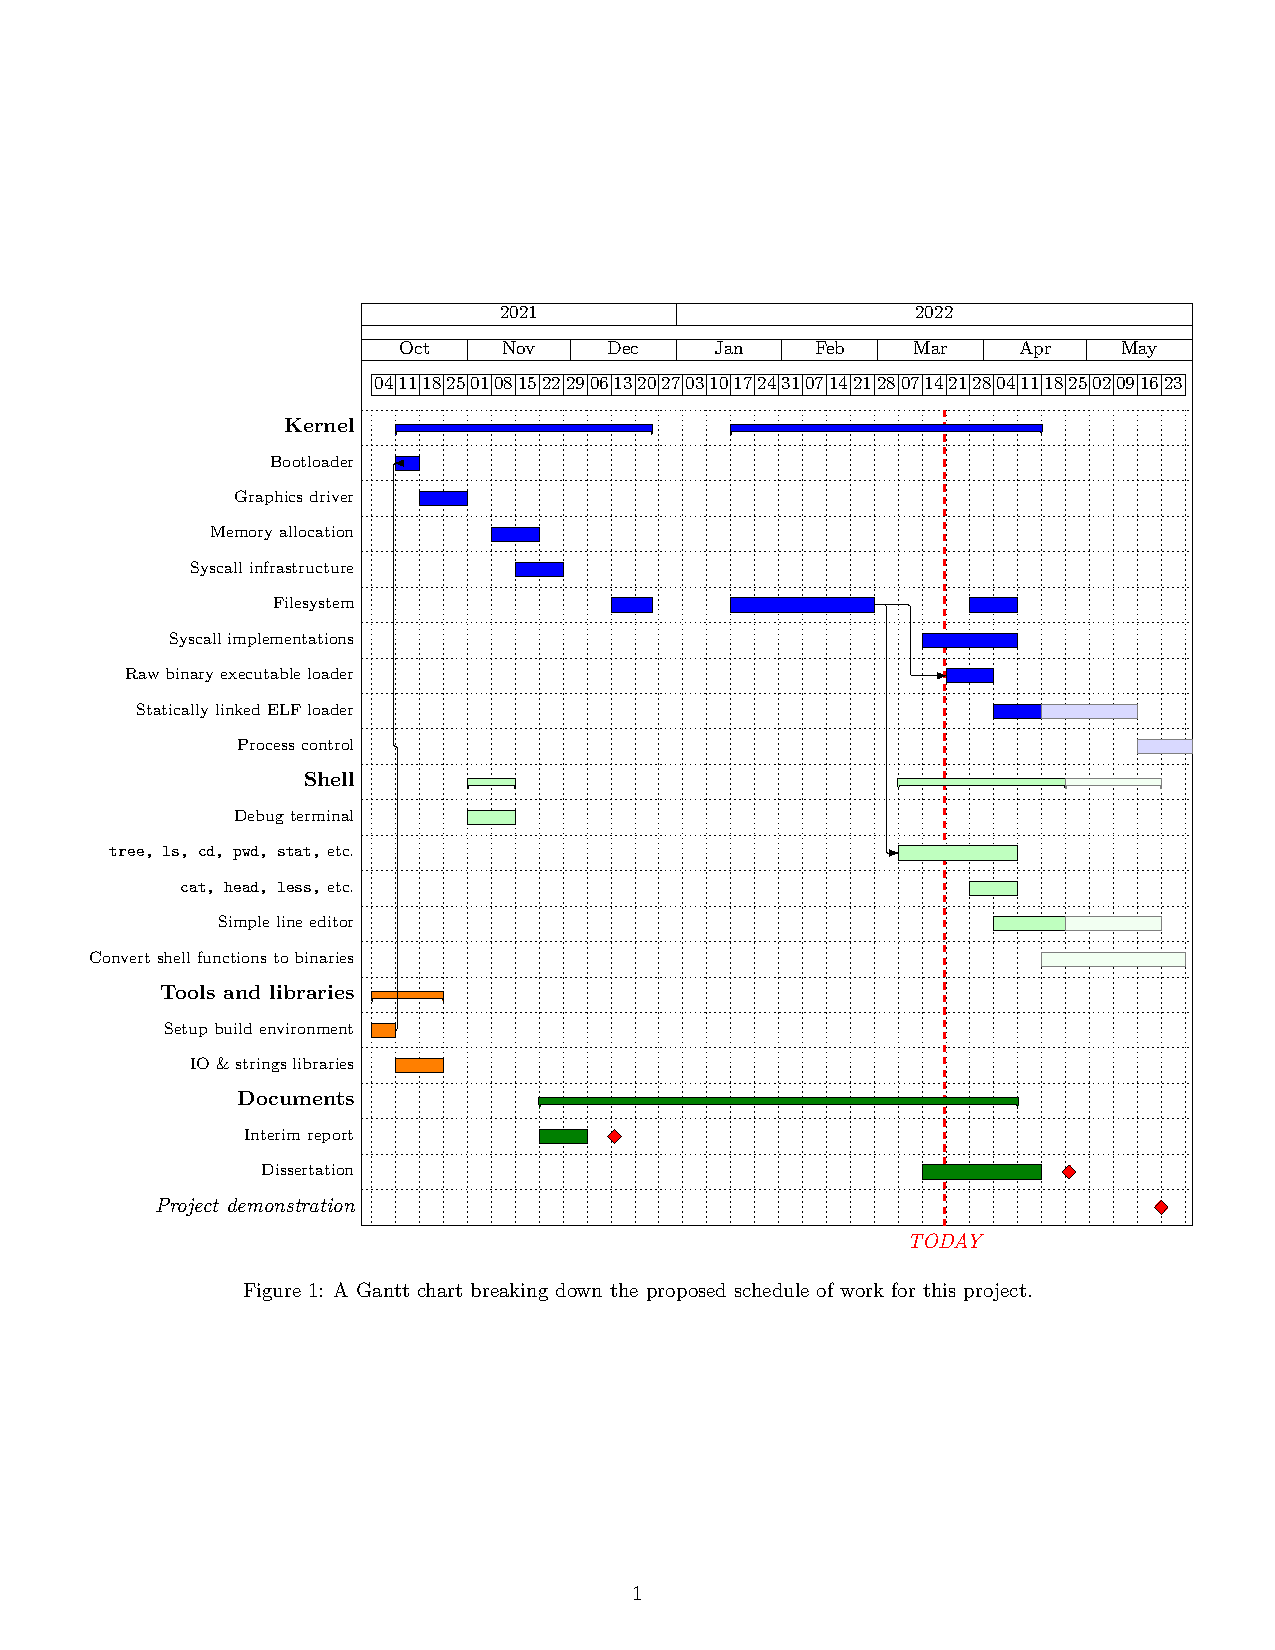
\includegraphics[width=0.95\textwidth]{build/gantt.pdf}
    \caption{Gantt chart showing the proposed breakdown of when I would do each
    task for the project.}
    \label{fig:gantt-chart}
\end{figure}


\section{Methodology}
\subsection{Setting up the build system}
For this project, I could not use a traditional compilation setup. Normally, a
program runs in a hosted environment, which means that it can use a standard
library for some basic functions. In the case of C code, this is \texttt{libc}.
My \gls{os} runs on \emph{bare metal}, so it cannot use any of the standard
header files provided by \texttt{libc}, which means that the entire C standard
library is unavailable. I still have access to some header files, including
\texttt{stddef.h} and \texttt{stdint.h}, as these are provided as part of the
compiler. There are other header files available in this \emph{freestanding}
environment, but these two were the main ones for the first stages of
development, since they define types such as \texttt{uint32\_t} and
\texttt{size\_t}.

In addition to the compiler flags needed for freestanding development, I also
needed a completely different compiler. This relates to the \emph{Architecture}
of the system running the compiler. The Raspberry Pi I used for this project
has an architecture of \texttt{Aarch64}, or 64-bit ARM, whereas desktop PCs are
usually \texttt{x86} or \texttt{x86\_64} architecture computers. This means I
needed a compiler that generates machine code for \texttt{Aarch64} based
systems. Such a compiler would be called a \emph{Cross-compiler} if it runs on
a different architecture compared with the machine code it produces.

\subsubsection{Cross-compilation terminology and tools}
\begin{itemize}
    \item \textbf{Build}: The architecture of the computer used to compile the
        program.
    \item \textbf{Host}: The architecture of the computer the program will run
        on.
    \item \textbf{Target}: The architecture the program builds for (only used
        when the program is or contains a compiler).
\end{itemize}
For this project I used the LLVM suite of tools, as it was designed to be a
cross-compiler first, so all of the tools (compiler, assembler, binary
manipulation tools, etc.) are capable of handling the required Aarch64 host
system. The compiler, \texttt{clang}, takes a command-line argument which indicates
the architecture of the host system (LLVM ignores the difference between host
and target, calling them both `target').
\subsection{Software tools used to aid development}
\subsubsection{Source code editing}
For editing the source code of the \gls{os}, I use the text editor
Vim~\cite{vim} with several plugins to assist me in writing correct code. I am
using the CoC extension~\cite{vim-coc} for autocompletion, and the clangd
language server~\cite{clangd} extension for CoC in order to provide source code
linting for C source files.

For source code formatting, I run the program
\texttt{clang-format}~\cite{clang-format} on the C source and header files. I
have defined a style guide for the project in a \texttt{.clang-format}
configuration file, which tells \texttt{clang-format} how to format my code.
This results in a consistent style throughout the entire project, causing the
source code to be easier to read and understand.

\subsubsection{\texorpdfstring{\glsxtrlong{rpi}}{RPi} 3 Emulator}
QEMU~\cite{qemu} is an emulator with out-of-the-box support for emulating the
host architecture. This means that on an \texttt{x86} machine, we can
emulate another \texttt{x86} machine. This isn't enough for emulating a
\gls{rpi}, as the \gls{rpi} uses the Aarch64 architecture. Thankfully, there is
a package on most linux distributions, ususally called something like
\texttt{qemu-arch-extra}, which adds support for other architectures. This
provides the program \texttt{qemu-system-aarch64}, which spins up an emulator
for Aarch64-based machines. The \gls{rpi} 3 is supported as a machine preset,
using the command line argument \texttt{-machine raspi3}.

The emulator can emulate everything about the \gls{rpi} except for the first
stage bootloader, which is the code that runs at the very start of the boot
process on a real \gls{rpi} and then loads the kernel (\texttt{kernel8.img}
for 64 bit mode). This bootloader is proprietary and runs on the \gls{rpi}'s
VideoCore GPU. I am not trying to develop a first stage bootloader, though, so
I do not need to worry about the lack of this functionality. The compiled
kernel is passed as an argument to the emulator when we start it
(\texttt{-kernel kernel8.img}). In the same way, we can give the SD card image
to the emulator, with the argument \texttt{-drive
file=sd.img,if=sd,format=raw}.

\subsubsection{Debugging}
GDB~\cite{gdb} is a debugger which can be used to debug executable programs.
Similar to QEMU only supporting one architecture by default, GDB only supports
running a program directly on the current machine. However, it does support
remote debugging with a commands once it has started (\texttt{target remote
URL:PORT}). Like with QEMU, there is an additional package which provides
support for additional architectures (\texttt{gdb-multiarch}). When we launch
QEMU, we can tell it to wait for a remote debugging session to connect before
it starts the emulator (using the commandline arguments \texttt{-s -S}). Once
QEMU is waiting for the debugger, we launch GDB (\texttt{gdb-multiarch
kernel8.elf} in a terminal) and then connect to the emulator as a remote
debugging client (using the GDB command \texttt{target remote localhost:1234}).

Now we can debug the \gls{os} kernel as if it is a regular program, using
breakpoints and disassembling it as we run through the execution. This is how I
debug the kernel when a new feature is not running as expected, and it allows
me to determine the cause of any issues more easily than a debug shell would
have done. Also, the debugger works without needing a working kernel, so I can
debug issues which cause the kernel to fail.

\subsubsection{Organising the build process}
When I first started this project, I was using CMake to automate the build
process. CMake is a tool which tries to automatically find the correct
dependencies required for compiling a project (the compiler, linker, and also
any libraries and included files can all be handled by CMake). Unfortunately,
CMake was causing issues with compiler and linker paths, and it was not
consistently finding the correct linker for the compilation of this project.

I then rewrote the build system using GNU Make (with a Makefile). This allowed
me to hardcode the correct compiler and linker for the build process, and I
haven't encountered any more issues with the compilation toolchain.

The top-level Makefile does not contain any rules to invoke the compiler
directly, and only handles the linking together of the compiled object files
into the final kernel. A separate Makefile is used to compile each source file,
and Make invokes itself recursively in each source directory for the
compilation.

The source files are kept separate from the object files and compiled kernel,
by putting all the results of compilation into a \texttt{build/} directory at
the top of the project (source files are located in \texttt{src/}). The object
files and final compiled binaries are also separated, with object files being
in \texttt{build/obj/} and binaries in \texttt{build/bin/}. Keeping the
directory structure organised in this way helps maintain an understanding of
the overall project structure as the project grows in size, as not keeping the
order in this way would result in quickly becoming overwhelmed by the sheer
number of files.

\section{Design}
\subsection{\texorpdfstring{\gls{os}}{OS} components block diagram}
\autoref{fig:os-block-diagram} is a diagram of how the different components of
the Unix \gls{os} fit together. It shows how user programs running on the
\gls{os} are supported by the \gls{os} components. The components mentioned
include user libraries, as well as various parts of the kernel, such as system
calls (see \autoref{sec:impl_syscalls}), the \gls{fs} (\autoref{sec:impl_fs}),
and the \emph{process control subsystem}.

\autoref{fig:os-block-diagram} is also a representation of one possible final
goal state of the \gls{os}, specifically a final goal state that is very
heavily influenced by Unix, but there will be different designs which the
\gls{os} could follow moving on after this project's timescale. A diagram in
the same style which more accurately represents the components that have been
implemented during this project is shown in
\autoref{fig:finished_block_diagram}.

The differences between the two designs, as well as one proposed path from this
project's result to the \emph{Unix structure}, can be seen in
\autoref{fig:block_diagrams_progression}.

\begin{figure}[htbp]
    \centering
    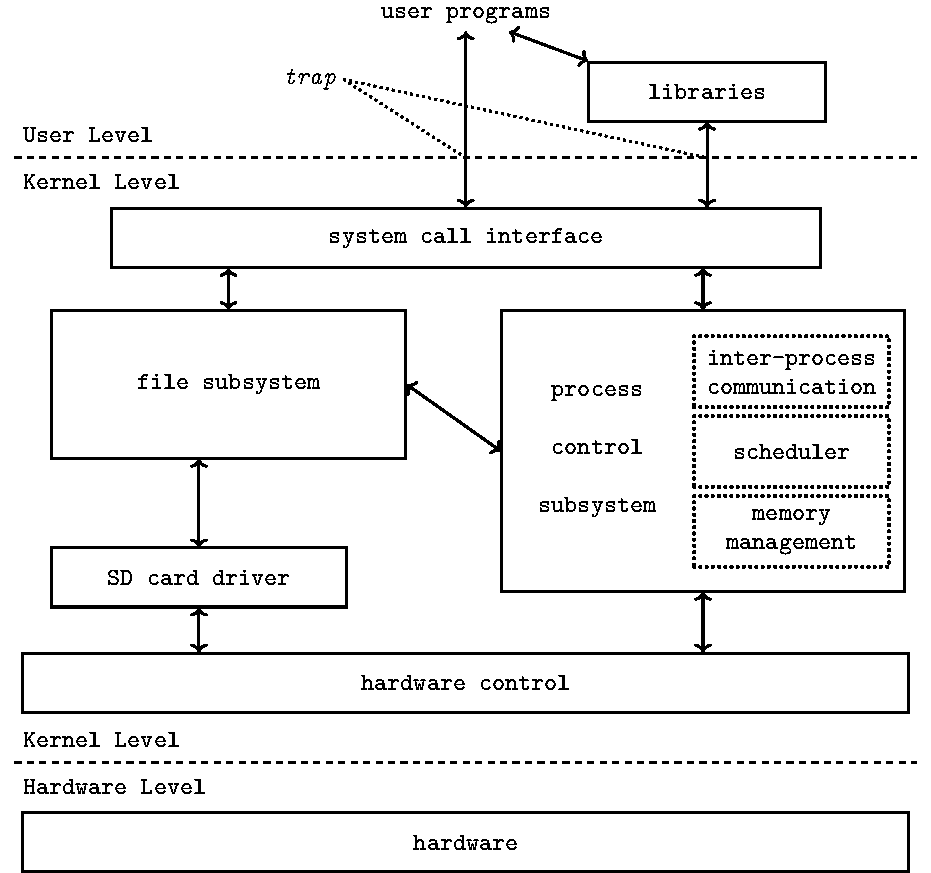
\includegraphics[width=0.8\textwidth]{build/os-block-diagram.pdf}
    \caption{A diagram of how the components of the Unix operating system
        interact with each other. Inspired by a diagram from a book on Unix
        (Figure~2.1 from~\cite{design-of-unix-os}). The versions of this
        diagram which are available online are low-resolution, so the version
        provided here is in a vector format, and this document's source code is
        available online~\cite{this-document}.}
    \label{fig:os-block-diagram}
\end{figure}

\begin{figure}[htbp]
    \centering
    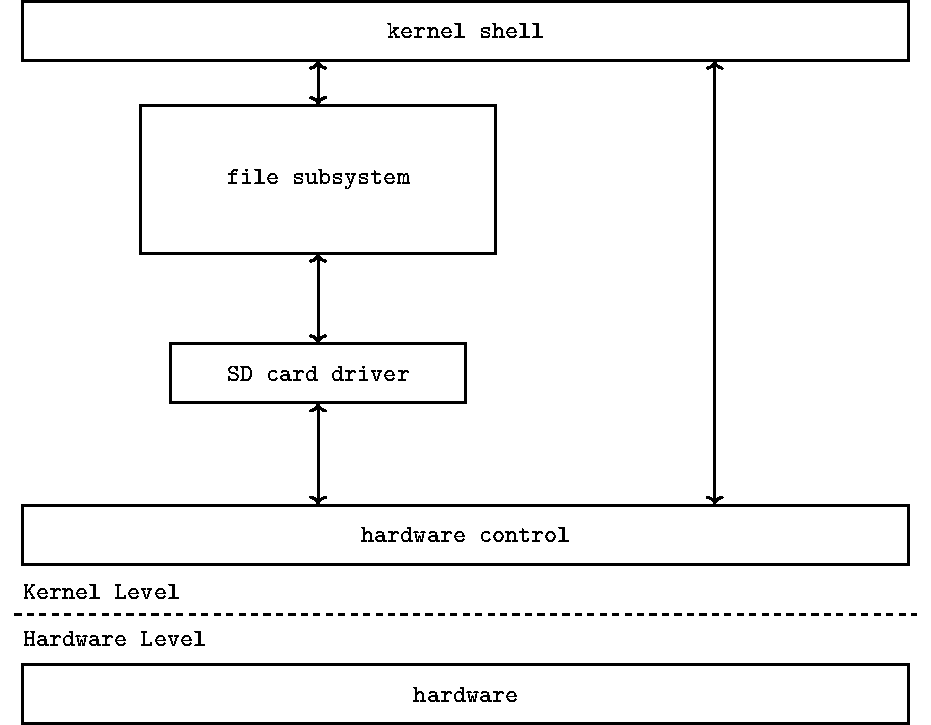
\includegraphics[width=0.8\textwidth]{build/finished-block-diagram.pdf}
    \caption{The structure of this project's \gls{os} at the end of the
    project.}
    \label{fig:finished_block_diagram}
\end{figure}

\begin{figure}[htbp]
    \centering
    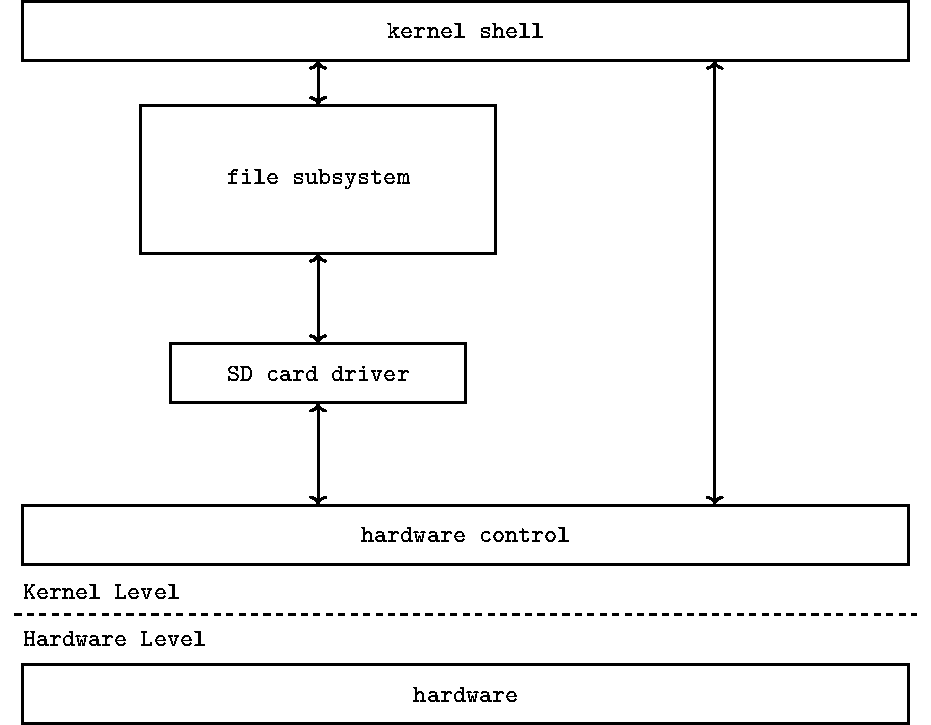
\includegraphics[width=0.32\textwidth]{build/finished-block-diagram.pdf}
    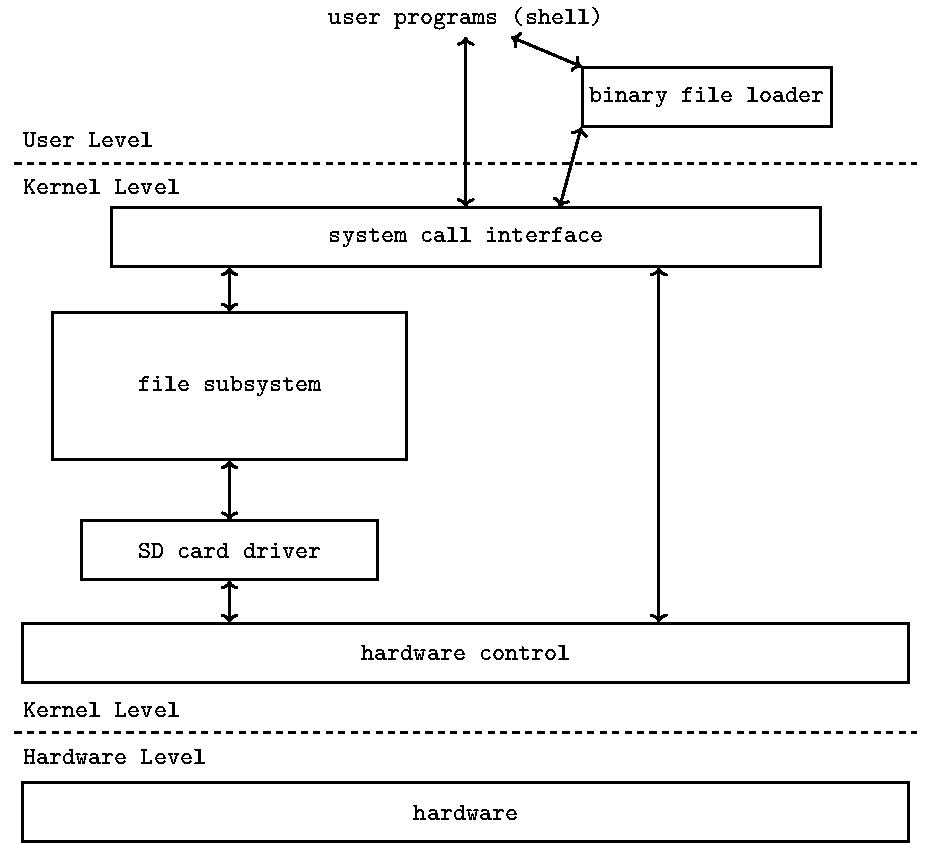
\includegraphics[width=0.32\textwidth]{build/nextstep-block-diagram.pdf}
    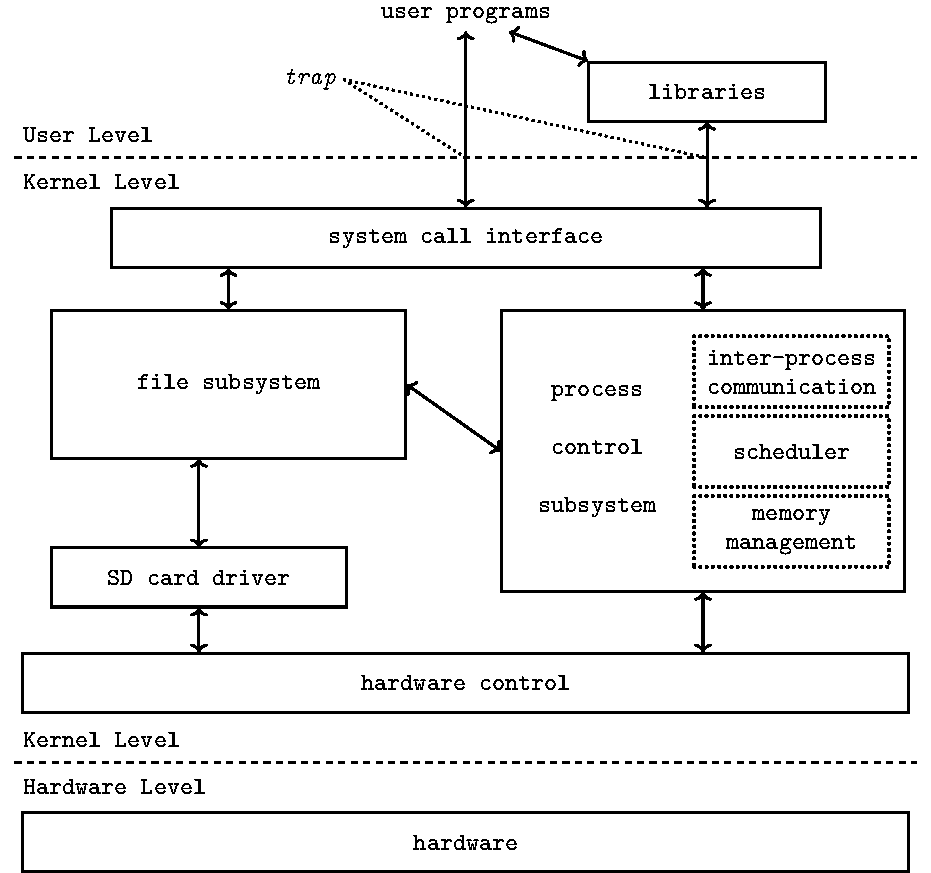
\includegraphics[width=0.32\textwidth]{build/os-block-diagram.pdf}
    \caption{Three diagrams showing a suggested development path the \gls{os}
    could take after this project. The end goal of this path is the structure
    of the Unix \gls{os}. The three diagrams are shown full-size in the
    appendix.}
    \label{fig:block_diagrams_progression}
\end{figure}

\subsection{User Interface and the graphics of the
\texorpdfstring{\gls{os}}{OS}}
The interface of the \gls{os} is the console. It is the text that is displayed
to the user from the \gls{rpi}. I will implement some quality of life features,
such as terminal scrollback, which allows the user to scroll up and see what
was printed to the terminal earlier. This feature reduces the need for a
terminal output pager such as \texttt{less}, which will not be implemented
until very late in the development.

The font I decided to use for the console is Bizcat~\cite{bizcat-font}. It is
an 8x16 bitmap font, and I converted it into a C source file as a constant
array. The font is easy to read at a screen resolution of 640x480, which gives
80 columns and 30 rows of text.

The original colorscheme of the console was solid white text on a completely
black background, but I found that this was too harsh to look at for long
periods of time. I changed both the background and foreground colours to what I
found more pleasant to read text from, with a very light grey text on a very
dark grey background. A comparison of the colorschemes can be seen in
\autoref{fig:console_colorscheme_comparison}.

\begin{figure}[htpb]
    \centering
    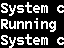
\includegraphics[width=0.45\textwidth]{figure/black.png}
    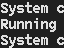
\includegraphics[width=0.45\textwidth]{figure/grey.png}
    \caption{The original colorscheme of the console (left) and the new
    colorscheme (right).}
    \label{fig:console_colorscheme_comparison}
\end{figure}

\section{Programming languages and compilation toolchain}
\subsection{Programming languages used}
From the beginning of this project, I had already decided to write the majority
of the code for the \gls{os} in C~\cite{c-programming-language}. C is primarily
a systems implementation language (making it perfect for writing an \gls{os}),
and I was already very familiar with it, having used it regularly for the past
5 years.

For some very low-level parts of the \gls{os}, I needed to specify the exact
order in which I wanted \gls{arm} instructions to be executed, so ARMv8
assembly was the natural choice, being the closest language to the machine code
that gets executed without actually being the machine code. Assembly language
allows preprocessor macros, so I did not have to manually align instructions to
4-byte boundaries anytime there was a change, and header file ``include''s
which allow register values to be abstracted away from the logic and replaced
with meaningful names. These features were used extensively in the bootloader
and in \autoref{sec:impl_cpu_setup} for explaining the values placed into
various \gls{cpu} registers.

\subsection{Problems with the original compilation toolchain}
At the start of development, I was using the GNU cross-compiler for bare-metal
\gls{arm} 64-bit targets, \texttt{gcc-aarch64-none-elf}. This was working but
the build system I was using at the time (CMake) was easier to configure using
clang/llvm as a cross-compiler. Also, the GNU cross-compilers are not available
in most Linux distributions' core repositories, so clang/llvm is much easier to
install, needing only the package manager of a Linux system.

Later in development, I was having difficulties maintaining the build system
which I had started the project with (CMake), as the intended usage is to
automatically detect the executables that should be used for compilation (the
cross-compiler, linker, etc.). This caused problems because if I modified the
status of my build computer, by installing some new packages for example, CMake
would detect and start using the wrong linker, causing the build process to
fail\footnote{I later discovered the cause of this. I had re-installed the
\texttt{gcc-aarch64-none-elf} cross-compiler, which resulted in the GNU
\gls{arm} 64-bit linker appearing before llvm's \texttt{ld.ldd}. CMake then
tried to use \texttt{gcc} (\textbf{not} the cross-compiler) to invoke the
linker, but the arguments for invoking the linker via \texttt{gcc} and
\texttt{clang} are different, so \texttt{gcc} was giving back an error, saying
that the \texttt{-T} argument was missing a parameter, and I was unable to
force CMake to call \texttt{ld.ldd} directly.}.

As a result of the problems I was having with CMake, I decided to use GNU Make
(with a \texttt{Makefile} instead of a \texttt{CMakeLists.txt}, calling the
\texttt{make} executable) instead. I created a Makefile for the project, and
this allowed me to hardcode the name of the compiler executable, and all the
tools needed to generate the compiled kernel image and SD card image. During
the implementation, as the number of source code files grew, I decided to start
using sub-make~\cite{sub-make} for compilation so that the main Makefile could
be kept simpler, so I moved the compilation commands into a separate Makefile
which handles each subdirectory of the main \texttt{src/} directory.

\section{The Kernel}
\subsection{Design}
\label{sec:kernel_design}
\subsubsection{Bootloader}
On the \gls{rpi} 3, the \gls{gpu} contains a first-stage bootloader which
automatically does most of the required setup for booting into an \gls{os}
kernel. However, the \gls{cpu} will not be setup completely, and so I will need
to write some code to set register values and verify that everything is as it
should be before we jump into the kernel \texttt{main} function. I will call
this code the `second-stage' bootloader.

\subsubsection{\texorpdfstring{\glsxtrshort{uart}}{UART} driver for keyboard
input and initial console output}
\gls{uart} is used on the \gls{rpi} for serial communication, with two
different \gls{uart} ports: a mini-UART and a full PL011
\gls{uart}~\cite{rpi-uarts}. The PL011 \gls{uart} is faster and more reliable
than the mini-UART, but it is disabled by default, enabling it disables
bluetooth, and it is more complex to program for. I will use the mini-UART to
debug the setup of the PL011 \gls{uart}, which will be used as the main serial
connection once it is enabled and working. I won't be using bluetooth in this
project, but future projects which expand on my code could switch back to the
mini-UART if they wanted to use the \gls{rpi}'s bluetooth chip.

Serial communication is used in this project as a means of interacting with the
\gls{os}, as I will not be implementing support for USB peripherals. All
keyboard input is expected to come through the serial port. I will also use the
serial port for debugging as I develop the graphics driver (see
\autoref{sec:design_graphics_driver}).

For the initial console output, I will implement a \texttt{printf} function for
formatted printing of characters, integers, hexadecimal numbers, and strings.
This will allow me to easily print the values of registers, so that I can make
sure that all values are as I expect during the boot process. The
\texttt{printf} function will be generic, so that I can use the same
\texttt{printf} function for both of the \glspl{uart} and also eventually for
the graphical console.

The \gls{os} will get keyboard input from the serial port, which will be
provided by QEMU, the \gls{rpi} emulator. QEMU uses VT100 escape
sequences~\cite{vt100} for its serial interface, so normal keys on the keyboard
(and shifted keys) are passed to the \gls{os} as the ASCII value of the
characters they represent.

\subsubsection{Graphics driver for displaying pixels on the screen}
\label{sec:design_graphics_driver}
Once I have a working serial terminal, I will implement a graphics driver for
interacting with the \gls{rpi}'s framebuffer. This will include a function for
setting individual pixels, a function for setting the entire screen to a
colour, and a function to display a bitmap to the screen at a given location.
With these functions, I will write functions for displaying characters to the
screen, with variables for the current position on the screen. I will convert a
bitmap font~\cite{bizcat-font} into a constant array of bitmap values, and the
character printing function can use the character as an index into this array
to get the bitmap to display to the screen.

The screen blanking function will use a \texttt{memset} function to set the
entire framebuffer to a given value, as this would be much faster than setting
each pixel individually. The bitmap function will use the pixel setting
function internally, and will use the bitmap to decide which pixels should be
set. Each of these functions is very simple on its own, and will be relatively
easy to implement, but once put together they will create the complex behaviour
required for displaying characters to the screen.

\subsubsection{System calls}
TODO: explain that syscalls are split into 2 different components: the
mechanism to allow for them and the implementations of the syscall functions
themselves.

\paragraph{System call mechanism using software interrupts}
The kernel will include a system call mechanism, which would eventually be the
way for processes (at the user level) to escalate privileges temporarily to
request that the kernel perform some action on their behalf. Processes and the
user / kernel level split will not yet be implemented, but I will implement
support for system calls to prepare for the time when they are needed.

The \gls{os} will use software interrupts to trigger a system call, with an
exception handler to interpret which system call function needs to be called.
On \gls{arm} \glspl{cpu}, a software interrupt is capable of changing the
\gls{arm-el}. In user-mode (once that is implemented) the \gls{cpu} would be in
\gls{arm-el} 0, and kernel code will execute in \gls{arm-el} 1. The software
interrupt will place the \gls{cpu} into \gls{arm-el} 1, entering kernel-mode,
and when the system call function returns, the exception handler will run an
exception return instruction, placing the \gls{cpu} back into the \gls{arm-el}
that it was in when the software interrupt occurred. This is how the system
call mechanism will allow the \gls{os} to separate user space from kernel space
while still allowing user-mode processes to perform operations that require
kernel permissions.

Each system call will be assigned a number, and I will copy these from Linux at
the start. Most Linux system calls will not ever be implemented, but having
some level of equivalence between this system and Linux system calls will
ensure that developer will feel confident that at least some of the knowledge
is transferable.

The system call exception handler will use the system call number to determine
which function to call. This will be done using a table in memory which maps
system call numbers to function pointers. The exception handler will lookup the
correct table entry and then call the function at the address it finds.

\paragraph{System call implementations}
The implementation of the system calls can be separated from the mechanism
which enables them to operate.
TODO: Expand this

\subsubsection{SD card driver}
In order to read data from the SD card on the \gls{rpi} (and write data back to
it), the \gls{os} will need to implement a driver for the \gls{rpi}'s eMMC
chip. The simplest way to do this will be to copy an existing driver for that
chip. I will take code from one of the related works~\cite{rpi-boot-gh}.

\subsubsection{exFAT filesystem}
The kernel will include an implementation of the exFAT filesystem. I considered
several different filesystems including FAT32, exFAT, and
YAFFS~\cite{yaffs-fs}. The exFAT filesystem's popularity was the reason I chose
it over YAFFS. The FAT32 filesystem seems simpler to implement than exFAT, but
I was not able to find a specification for it online, whereas the exFAT
official specification is available on Microsoft's documentation
website~\cite{exFAT-specs}. Having a single source for the filesystem
specification gave me more confidence that different tools would work together.
Also, the exFAT filesystem is partially supported on Linux systems (FAT32 is
not as well supported), and I am developing the \gls{os} on Linux.

The file system implementation will need several features in order to work as
the main filesystem of this \gls{os}. These are listed below, using terminology
that will be explained in \autoref{sec:impl_fs}.

\begin{itemize}
    \item Read the `superblock' of the SD card
    \item Interpret the FAT table to follow cluster chains
    \item Read directory entries
    \item Search a directory for a file according to its name
    \item Read the contents of a file
    \item Write to a file and correctly update its metadata for size and
        modification time
\end{itemize}

\subsection{Implementation}
\subsubsection{Bootloader}
The second-stage bootloader\footnote{The `bootloader' is more accurately
described as boot code, since it does not do any loading of the kernel from
disk, the traditional task of a bootloader.} is written in \gls{arm} assembly
code. This is because the bootloader performs the necessary setup in order to
get the \gls{cpu} and memory into a state in which code written in C can be
run. Once the bootloader has finished this setup, it jumps into the kernel main
function (written in C) straight away.

First, the bootloader stops all but one of the \gls{cpu} cores. The current
state of the \gls{os} does not support simultaneous multiprocessing with the
multicore \gls{cpu} on the \gls{rpi}. This first step effectively converts the
4-core \gls{cpu} into a single-core \gls{cpu} by putting cores 1, 2, and 3 into
infinite `do-nothing' loops, leaving only core 0 to execute code.

Next, the boot code gets the current \gls{arm-el} from the \gls{cpu}. The
\gls{arm-el} is stored in a special \gls{cpu} register on \gls{arm}
\glspl{cpu}, called \verb!CurrentEL!. On the \gls{rpi} this should always be 2,
but I also wrote code to handle the case where it is 3. If the \gls{arm-el} is
3 then the boot code sets the needed registers and safely transitions the
\gls{cpu} into \gls{arm-el} 2 in the same way as described below.

\paragraph{Changing the \texorpdfstring{\glsxtrlong{arm-el}}{Exception Level}}
Once the boot code verifies that it is executing in \gls{arm-el} 2, it prepares
to change to \gls{arm-el} 1, the level that the kernel code will run in. It
sets important registers, such as the exception vector table (used by the
system call mechanism) and the exception return address (the address of the
code to execute once the \gls{cpu} switches to \gls{arm-el} 1). It also ensures
that \gls{arm-el} 1 is executing in 64-bit mode.

Once all the parameters are set correctly, the bootloader executes an exception
return instruction (\verb!eret!). Exceptions are the only way to increase the
\gls{arm-el} on an \gls{arm} \gls{cpu}, and returning from exceptions is the
only way to reduce the \gls{arm-el}. The exception return instruction changes
the \gls{cpu} into \gls{arm-el} 1 and resumes execution at the address of the
\gls{arm-el} 1 code.

\paragraph{The floating point / vector registers}
Once I started to implement the function \verb!printf!, which is a
\emph{variadic} function\footnote{A variadic function is one with a variable
number of arguments}, I started to experience strange behaviour. I debugged the
compiled kernel using remote debugging in GDB, and discovered that upon
entering the \verb!printf! function, the executing kernel would jump to an
address near \texttt{0x0}, the beginning of memory. This meant that an
exception was occurring and the \gls{cpu} was going to a position in the
\emph{Exception Vector Table}. I determined from the offset into the exception
table that the exception was permission related.

Looking at the first instructions in the disassembly of the \verb!printf!
function, I saw that the function was accessing registers I did not recognise,
labeled \texttt{Qn} instead of \texttt{Xn}. After some research I determined
that the \verb!printf! function was trying to use the 32 floating point
registers of the \gls{cpu} to store the variadic argument list, but the
floating point registers were disabled by default.

The solution was to enable the floating point registers after switching to
\gls{arm-el} 1, by setting some bits in one of the system registers. Setting
those bits enabled the floating point registers (also called vector registers)
and enabled the use of variadic functions in the C code.

\subsubsection{System Calls}
\label{sec:impl_syscalls}
The system call interface required writing an exception handler and an
\emph{Exception Vector Table} The \emph{Exception Vector Table} is a
table in memory which gives the \gls{cpu} instructions to execute for each
different type of exception that can occur while it is running. These could
include hardware interrupts such as timers, software interrupts (like the
system calls we are interested in), or more serious errors like invalid
instructions or insufficient permissions for an operation. I originally wrote
the Exception Vector Table using outdated documentation, so the padding between
entries was incorrect. I fixed this issue, and placed a jump instruction in the
software interrupt exception entry. This branched the \gls{cpu} to the
exception handler that I wrote.

I wrote the exception handler for software interrupts in \gls{arm} assembly
code, the same as the Exception Vector Table. First, it checks that the
instruction that generated the exception was the supervisor call instruction,
\verb!svc!. Then it checks the argument of that instruction -- we only want
exceptions where the argument was 0. After checking that the exception was
indeed a system call, the exception handler gets the system call number and the
(up to) 6 arguments and places them into the first 7 general purpose registers.
It reads an index into a named table (\verb!sys_call_table!) and uses the
address it reads as a function pointer, calling the function. This is the
mechanism used to identify the correct system call function from just the
system call number.

Also in the assembly code for system calls is an indirect system call function
(\verb!syscall!). This function is equivalent to the Linux function
\verb!int syscall(long number, ...)!, and is the intended way for C code to
invoke a system call. Eventually I would write named wrapper functions for the
common system calls, but for now the way that C code would run the
\texttt{read} system call, for example, would be as shown in
\autoref{lst:syscall-example-read}.

\begin{lstlisting}[language=C, caption={How some C code would invoke the system
                   call \texttt{read} in the current implementation.}, float,
                   label={lst:syscall-example-read}]
extern int syscall(long nr, ...);
// read syscall is syscall number 0
// fd is a file descriptor
// buf is a void pointer to a buffer large enough to read to
// count is the number of bytes to be read
syscall(0, fd, buf, count);
\end{lstlisting}

\subsubsection{\texorpdfstring{\gls{cpu}}{CPU} setup}
\label{sec:impl_cpu_setup}
When the kernel starts, the \gls{cpu} will either be in \gls{arm-el} 2 or
\gls{arm-el} 3 (The \gls{rpi} only supports \gls{arm-el} 2 but I have written
code to support \gls{arm-el} 3 just for completeness). The boot code of the
kernel checks the current \gls{arm-el} and runs some code to put the \gls{cpu}
into \gls{arm-el} 1. The code sets up the system registers correctly to fake
the \gls{cpu} returning from an exception. When the registers are correctly
set, the \gls{arm} instruction \texttt{eret} is run, and the \gls{cpu}
``returns'' from the ``exception handler'', jumping into the kernel code and
entering into \gls{arm-el} 1. This is done in this way because exceptions are
the only way to change \gls{arm-el}, and the only way to reduce the
\gls{arm-el} is to perform an exception return (\texttt{eret}).

\subsubsection{exFAT \texorpdfstring{\gls{fs}}{Filesystem}}
\label{sec:impl_fs}
I took an existing driver for interfacing with an SD card (via the \gls{rpi}'s
eMMC controller) and integrated it into the kernel. This code defines a
structure called a \verb!struct block_device!. I also copied some \gls{fs} code
from the same related work~\cite{rpi-boot-gh}, but most of the code for the
\gls{fs} I wrote by myself.

I first created a function to read the `superblock' of an exFAT system. The
superblock is the first block of the disk partition, and contains some critical
information for interpreting the information on the rest of the disk. The
structure used to store this information and the declaration for the function
are both sown in \autoref{lst:exfat-read-superblock}. The function is called
\verb!exfat_read_boot_block()! because sometimes the superblock is referred to
as the `boot block' (although ususally only when talking about disks instead of
\glspl{fs}).

\begin{lstlisting}[language=C, caption={The structure used to represent the
                   exFAT superblock information, and the declaration of the
                   function used to read it}, float,
                   label={lst:exfat-read-superblock}]
struct exfat_superblock {
    uint64_t partition_offset;
    uint64_t volume_length;
    uint64_t sectorsize;  // Bytes per sector
    uint64_t clustersize;  // Sectors per cluster
    uint32_t fat_offset;
    uint32_t fat_length;
    uint32_t clusterheap_offset;
    uint32_t cluster_count;
    uint32_t rootdir_start; // First cluster of the root directory
    uint32_t volume_serialnumber;
    uint16_t fs_revision;
    uint8_t  fat_cnt;  // Number of FAT tables
    uint8_t  use_percent;
    // Volume flags
    uint8_t active_fat;  // Which fat is active
    bool volume_dirty;
    bool media_failure;
    bool clear_to_zero;
};
int exfat_read_boot_block(struct block_device *, struct exfat_superblock *);
\end{lstlisting}

There is also a function which takes a cluster index and returns the index of
the next cluster in that cluster's cluster chain. This information is retreived
by reading the \gls{fat} section on the volume (see section 4.1
in~\cite{exFAT-specs}). The function signature is shown in
\autoref{lst:exfat-read-fat}.

\begin{lstlisting}[language=C, caption={The function which is used to get the
                   cluster index of the next cluster in a cluster chain},
                   float, label={lst:exfat-read-fat}]
static uint32_t fat_idx_to_cluster_idx(struct block_device *dev, struct
        exfat_superblock sb, uint32_t fat_idx);
\end{lstlisting}

The next structure on an exFAT volume that needs to be interpreted is the
directory. Directories primarily contain information about files, but can also
contain some special entries. These are all stored in `directory entries' (see
sections 6 and 7 in~\cite{exFAT-specs}). The information for a directory is
stored in a \verb!struct exfat_directory_info!, and information describing a
single directory entry is stored in a \verb!struct exfat_dirent_info!. These
are both defined in \autoref{lst:exfat-dirent-structs}.

\begin{lstlisting}[language=C, caption={The structures which describe
                   directories and directory entries on an exFAT volume},
                   float, label={lst:exfat-dirent-structs}]
struct exfat_directory_info {
    struct block_device *bd;
    struct exfat_superblock super;
    uint32_t start_cluster; // First cluster of the directory
};

struct exfat_dirent_info {
    struct exfat_directory_info *parent;
    uint32_t direntset_idx;  // Index into the "Directory"
    // The importance, category, and type code represented in the same way as
    // on disk.
    enum EXFAT_DIRENT_TYPE type;
    bool in_use;  // The in_use bit of the entrytype field can change
    union {
        struct exfat_dirent_bitmap_chunk bitmap;
        struct exfat_dirent_upcase_chunk upcase_table;
        struct exfat_dirent_vollab_chunk volume_label;
        struct exfat_dirent_file_chunk file_metadata;
        struct exfat_dirent_volguid_chunk volume_guid;
        struct exfat_dirent_strext_chunk stream_extension;
        struct exfat_dirent_fname_chunk filename;
        struct exfat_dirent_vendor_guid_chunk vendor_guid;
        struct exfat_dirent_vendor_alloc_chunk vendor_alloc;
    } entry_data;
    // If the dirent doesn't point to another cluster chain, then data_length
    // will be 0.
    uint32_t first_cluster;
    uint64_t data_length;
};
\end{lstlisting}

A function in the exFAT driver, \verb!exfat_read_directory_entry()!, is used to
read and interpret a single directory entry. Its single argument is a pointer
to a \verb!struct exfat_dirent_info!, which is already filled with the
information that is needed to identify a single directory entry in a directory.
The function fills the rest of the fields.

Another function, \verb!exfat_readdir_fromblock()!, takes a block device (the
SD card) and the address of a block which is the beginning of a directory, and
reads the entire directory. It stores each file from the directory in a
\verb!struct dirent!, partially defined in \autoref{lst:dirent-struct}. The
\verb!dirent! structure contains a \verb!next! pointer, so the function joins
all of the files into a linked list data structure, and returns the first file.

\begin{lstlisting}[language=C, caption={The dirent struct, which stores
                   information about files}, float, label={lst:dirent-struct}]
// Struct representing a file
struct dirent {
    struct dirent *next;  // The next file in the directory
    char *name;  // Filename
    uint32_t byte_size;  // Size of the file
    uint8_t is_dir;  // Is this file a directory?
    ...
};
\end{lstlisting}

A distinction is made between a directory entry and a file. A directory entry
may not be associated with a file, and each file will have at least three
directory entries associated with it. The \verb!exfat_dirent_info! structure
refers to a single directory entry, whereas the \verb!dirent! structure
describes a single file. The \verb!exfat_readdir_fromblock()! function reads
directory entries in a loop, ignoring those not associated with files. It reads
all of the entries for each file, then creates the \verb!struct dirent! and
appends it to the linked list. When it reaches the `end of directory' directory
entry the function returns.

\subsubsection{Graphics driver}
\label{sec:impl_graphics}
For graphics, I created a simple library for manipulation of the framebuffer.
In order to print characters to the screen, I converted an 8x16 bitmap
font~\cite{bizcat-font} into a constant array definition in a C source file. I
then wrote a function to print a character from this array onto the
framebuffer, and I added global variables which keep track of the current
character position on the screen.

When the console reaches the end of a line, it moves to the start of the next
one. When it gets close to the bottom of the screen, the entire screen moves up
by one line each time the line wraps or a newline is printed. This is done
using a function that swaps rectangles on the framefuffer. First, the top row
is cleared, then each row of text on the screen is treated as a rectangle and
swapped with the line above it. The final result of this is that every line of
text moves up by one row, except the row already at the top, which is removed
(since it would go off the screen if it moved up).

\subsection{Evaluation}
Overall, the kernel met the requirements that I set out in
\autoref{sec:kernel_design}. Most of the components designed for the kernel
have been implemented. The ones which have not been fully implemented are
either almost finished and lacking some other piece of the \gls{os}, or the
groundwork has already been laid to make developing the features easier. This
was done to help new developers to more easily understand the source code of
the project.

\subsubsection{Bootloader}
The bootloader is robust and reliable, starting the kernel main function every
time the \gls{os} boots. It sets up the \gls{cpu} into the correct
configuration, following the kernel's current requirements.

\subsubsection{System call mechanism}
The interface to system calls is well-implemented. The wrapper function used to
invoke a system call checks that the system call number is within the valid
range of numbers, preventing unnecessary software interrupts from being
generated. The complex mechanism required for properly managing system call
generation and handling has been broken down into logical parts which are each
small enough to be easily understood.

\subsubsection{System call implementations}
\label{sec:eval_no_syscalls}
There are currently no system call functions in the \gls{os}. The table which
is used by the system call exception handler is in place, so once the system
call functions are written they can easily be dropped into the table and then
immediately those system call numbers will start to function.

TODO: refer back to second aim of the project.

\subsubsection{Filesystem}
The exFAT \gls{fs} was only just implemented. Reading directory entries works,
but there aren't many functions built on top of that to allow for more abstract
access to the \gls{fs}. The virtual filesystem abstraction is severely lacking
in the current version of the \gls{os}. All code which interacts with the
\gls{fs} directly uses exFAT-specific functions. This limits both ease of
programming with the \gls{fs}, and the overall usefulness of the \gls{fs}.

I started to move towards having a simple virtual \gls{fs} abstraction in
recent development by creating several of the functions presented by the
\verb!struct fs! structure. These include a version of \texttt{fopen},
\texttt{fread}, and \texttt{fclose}, which are functions needed for reading
files.

I started to write the exFAT-specific version of \texttt{fread} very recently
in development. The function declaration is shown in \autoref{lst:exfat-fread},
along with versions of \texttt{fopen} and \texttt{fclose}. The arguments of the
functions are different from the standard arguments to these functions. This
was changed to make the implementation of the functions easier, because the
\verb!struct dirent! already points directly at a file, whereas a string
representing a file path can be difficult to interpret. Unfortunately, this
change just made it more difficult to write code which uses the functions,
since the calling function now needs to do the job of converting a path into a
\verb!dirent! structure.

\begin{lstlisting}[language=C, caption={Function declarations of the exFAT
                   versions of \texttt{fopen}, \texttt{fread}, and
                   \texttt{fclose}.}, float, label={lst:exfat-fread}]
FILE *exfat_fopen(struct fs*, struct dirent*, const char *mode);
size_t exfat_fread(struct fs *, void *ptr, size_t byte_size, FILE *stream);
int exfat_fclose(struct fs *, FILE *fp);
\end{lstlisting}

\subsubsection{Testing}
The test coverage of the kernel is currently very limited. I wrote enough tests
to determine that the testing system works and intended, then after that no
more tests were written. I should have been writing unit tests for every kernel
component, but instead most of them are effectively untested.

The lack of testing provides a great opportunity for new developers to become
familiar with the project. Writing tests for an existing component would give a
new developer very good in-depth knowledge of how that component works. A
developer who enjoys writing unit tests would be able to learn the entire
kernel just from writing tests. The testing could even be expanded to
components of the shell, which would allow a new developer to both improve the
reliability of the \gls{os} and learn how it works, priming them to start
creating new features.

\subsubsection{Kernel / user space}
The \gls{os} features no separation between \emph{kernel space} and \emph{user
space}. Everything that runs under the \gls{os} is effectively kernel code,
including the shell. Ideally, the shell would run at a lower \gls{arm-el} than
the kernel (i.e. \gls{arm-el} 0), giving it reduced permissions to access
hardware and execute restricted instructions (such as stopping the \gls{cpu}).
However, doing this would require system calls to be available to the user mode
shell, and (as mentioned in \autoref{sec:eval_no_syscalls}) there are currently
no system call functions implemented in a working state. Therefore, creating a
separation between kernel code and user code is not currently possible. This
will be a high priority feature once system calls are available.

On the other hand, this feature could be used to drive the implementation of
system call functions. A developer could start work on getting non-critical
code to run in \gls{arm-el} 0, and then implement system calls as they are
required. This would be possible because the system call mechanism is already
implemented, and the only thing needed to get a given system call working is an
implementation of the function. A small amount of experimentation will also be
required to discover if any additional changes need to be made to the boot code
to get the \gls{cpu} to run in \gls{arm-el} 0 correctly.

\section{The Shell}
The design of the shell is important. If it is done correctly, developers who
are comfortable using a shell will immediately feel at home when they sit down
in from of this \gls{os}. A simple and intuitive shell will give a good first
impression to the project's code, which is important for the project's aims.

\subsection{Design}

\subsubsection{Commands as functions}
In the initial implementation, I will develop the shell as a part of the
kernel, and all of the commands will be functions built into the final compiled
kernel. I will do it this way because it is simple, and my \gls{os} will not
have a binary file loader at this stage, which would be needed for loading
external versions of commands. The downside of using this method is that any
new commands or changes to commands would require a recompile and rebuild of
the entire kernel, but so far building the kernel from scratch is a relatively
quick process.

Commands in the shell will be functions in the shell source code files. The
functions for commands will all share the same function signature, which will
be the same as the function signature for a \texttt{main}
function~\cite{c-main-func}. This will mean minimal changes would be needed to
eventually turn each command into its own executable, with the binaries being
stored on the filesystem (in a \texttt{/bin} directory). This change will be
the natural next step from what I create, so I am designing my shell
implementation with that in mind from the start.

\subsubsection{The shell loop}
The logic of an interactive shell is quite simple. It consists of an infinite
loop:

\begin{itemize}
    \item Read a line from the keyboard
    \item Split the line into words by spaces
    \item Determine which command, if any, the first word matches
    \item Execute the correct command
    \item Repeat this process forever
\end{itemize}

The shell needs to get user input on a line-by-line basis, since each command
starts at the beginning of the line and ends at the newline character. In the
first iteration, I will store the text input in a fixed-size buffer, meaning
that there will be a maximum size for an input line. I will set this maximum
size to a reasonable value such that it will not cause any problems, and I will
leave this problem to fixed in a future update to the shell's user input
functions.

I will split the line by spaces and place the words into a `vector',
passed to the commands as the argument \texttt{argv}.

\subsubsection{The commands}
I will create several commands, starting with the simplest and most essential
ones. The \gls{os} will need a way to shutdown the \gls{rpi}, so I will
implement a \texttt{shutdown} command. I will write a \texttt{pwd} command to
print the current working directory, as this will be a very simple (and also
useful) operation. When I write the filesystem, I will create a function for
printing the contents of directories (\texttt{ls}), and also a recursive
version of this, \texttt{tree}, shich shows an entire directory structure in
context.

Once I have implemented enough of the filesystem to get file contents from the
SD card, I will create a \texttt{cat} command to print files to the screen.
Finally, a command for getting file attributes, like \texttt{stat} on Linux
systems. On Linux systems, \texttt{stat} is implemented via a system call
(\texttt{fstatat}), so this command could be rewritten using that if a future
development creates that system call.

\subsubsection{Executable file loader}
One feature that would significantly improve the shell would be the inclusion
of a binary file loader. This could either support only raw binary files, or
statically compiled \gls{elf} files. A file loader would not be possible
without first implementing file reading in the filesystem, so this would be a
very late feature to start implementing if I put it into the \gls{os}.

For loading \gls{elf} files, I would implement a basic \gls{elf} parser to
extract the instructions from the file and put them into memory. The loader
would then determine where the entry point is, setup the stack and \gls{cpu}
registers, then finally jump to the entry point.

The process would be the same for loading raw binary files, except that the
entry point would be fixed. There would also be no need to extract the
instructions from the \gls{elf} structure, just loading the instructions from
the filesystem and then jumping into the loaded file contents.

\subsubsection{Rewrite commands using system calls}
Many of the commands I will implement would benefit from using some standard
system calls, but I will not have implemented any system calls by the time I
create the commands. Rewriting these commands to use the system calls would be
a nice-to-have feature. It would also give an incentive to implement the
common system calls, as I would be developing system calls I need at the time.

Some commands which would benefit from this would be \texttt{ls} (system call
\texttt{getdents}), \texttt{stat} (\texttt{fstatat}), and \texttt{cat} (which
would benefit from the system calls \texttt{open} and \texttt{read}). The
\texttt{printf} function could also be rewritten to use the system call
\texttt{write}, writing to a file descriptor which represents the graphical
console.

\subsubsection{Replace the shell and all commands with separate executables}
As a follow up to including a binary file loader in the shell, I could also
completely separate the shell and kernel. This would allow me to modify the
shell, which will be growing in size, without recompiling the kernel, which
will also be growing in size. The individual compile-times of both the shell
and the kernel would be effectively cut in half, allowing for much more rapid
iteration and development of both.

With the shell separated from the kernel, the kernel would load the shell from
the filesystem on boot (using the binary file loader). The commands could also
be moved to their own executables, and placed into some common directory,
likely \texttt{/bin/}. The shell would search this directory for filenames when
it is trying to find executables that match input lines. This hardcoded
directory would eventually be replaced by an environment variable
\texttt{PATH}.

Doing this would allow modification of the commands available on the system
without recompiling the kernel, restarting the \gls{os}, or even restarting the
shell.


\subsection{Implementation}
\subsubsection{Getting input from the keyboard}
The shell needs to get input from the keyboard line-by-line, so the terminal
can buffer the current line as it is being typed. A buffer of a fixed size is
created on the stack when the shell is started. The terminal uses a
\texttt{getc()} function to get one character from the serial port. When
\texttt{getc()} returns a newline character, the shell's input line buffer gets
tokenised, splitting it by spaces. The function \texttt{strtok()} (from
\texttt{string.h}) is used for this.

The addresses of the strings containing the tokenised words from the line are
placed into an array, which is the member `\texttt{argv}' of a \texttt{struct
command\_args}. The total number of words in the line is placed into that
struct's member `\texttt{argc}'. The member variable `\texttt{envp}' is set to
a pointer to the global \texttt{struct process\_env} of the kernel. This struct
contains all the miscellaneous information that commands may need, such as the
current working directory and the return value of the previous command. Once
the \gls{os} implements the concept of user and kernel space, only a subset of
this struct would be passed to commands, and then the commands would need to
use system calls (see \autoref{sec:impl_syscalls}) to access that information.

\subsubsection{Storage of enabled commands}
The shell's memory contains a linked list which contains all of the enabled
commands. The commands are described by a structure called a \texttt{struct
shell\_command}, with the structure definition shown in
\autoref{lst:struct-shell-command}. The member \verb!cmd_str! is a string
containing the word that is used to invoke that command, and \verb!fun! is a
function pointer to the function that will be used whenever the first word of
an input line is equal to \verb!cmd_str!.

\begin{lstlisting}[language=C, caption={The definition of the
                   \texttt{shell\_command} struct}, float,
                   label={lst:struct-shell-command}]
struct shell_command {
    int (*fun)(struct command_args);
    const char *cmd_str;
};
\end{lstlisting}

\subsubsection{Shell commands as functions}
In the current implementation, all of the commands that are available to the
shell are functions in the source code of the kernel. The function signature of
the command functions is shown in \autoref{lst:shell-func-signatures}, as
\verb!command_function()!. The function \verb!add_command()!, also declared in
\autoref{lst:shell-func-signatures}, takes a string and a function pointer and
creates a \verb!struct shell_command! from them, adding it to the shell's
\verb!struct shell_cmdlist! (the linked list). The function \verb!shell_init()!
calls \verb!add_command()! once for every shell command, initialising the shell
to prepare it for running commands.

\begin{lstlisting}[language=C, caption={The signatures of some important
                   functions for the shell}, float,
                   label={lst:shell-func-signatures}]
int command_function(struct command_args);
int add_command(const char *cmd_str, int (*fun)(struct command_args));
int shell_init();
\end{lstlisting}

\subsection{Evaluation}
Overall I am pleased with the progress I have made with the shell, but I have
not made as much progress as I originally hoped for. I think this was due to
the kernel containing some surprises that I did not consider or have the
knowledge to pre-empt at the beginning of the project.

The modular design for creating shell commands was a good implementation
choice. It is very simple to create new commands and get them working with the
shell -- this will be enticing to developers who see how easy it is to create a
simple utility function\footnote{A \emph{Hello world} example function could be
placed into the \texttt{README.md} of the git repository to showcase how easy
it is.}. All that is needed is a wrapper function with the correct signature
and a name for the command.

The argument to the shell command functions is very similar to the arguments
that a \texttt{main()} function would take once the shell moves to the commands
being individual executables. The first two arguments\footnote{The first two
members of the structure} are exactly the same (\verb!int argc, char *argv!).
This similarity will make the transition to commands as separate executable
files much easier since the command function can be copied directly to a main
function and then compiled on its own.

The third member of the \verb!command_args! structure, \verb!envp! is badly
named -- it doesn't contain any environment variables. In the future, the data
which is currently stored in this \verb!struct process_env! will be stored in a
table in the kernel, and tracked on a per-process level. Shell commands will
use system calls to access the same information.

One command that I would like to implement in the near future is a basic text
editor. This would be a line-oriented editor, with the basic functionality of
\texttt{ed}~\cite{ed}, the Unix text editor. Writing a simple text editor will
require the ability to write and create files, so this would prompt me to
implement that functionality into the exFAT \gls{fs}.

A final extension to the shell would be to include some shell language
features. This will effectively make the shell program an interpreter for an
\texttt{sh}-like language. The interactive version of the shell would become a
Read-Evaluate-Print-Loop (REPL) for the interpreter. Implementing a full
interpreter is obviously well outside of the scope of this project, but adding
these features would turn the shell into something that could be used for
scripting, which would complement the \gls{os} nicely, and would make it seem
like a much more complete package. The inclusion of a scriptable shell would
also be an attractive feature to many would-be new kernel developers, which
links back to one of the main aims of this project.

\section{Evaluation and External Aspects}
\subsection{Code style consistency}
The consistency of my coding style was not good over the course of this
project.

At the beginning of the project, I was writing functions with return
type \verb!ERROR_TYPE!, which was an alias of \verb!size_t!. Every possible
error was assigned a unique value (in an unmaintainable way), and for each
component there would be a unique success value.

Once \texttt{errno.h} was created, I started using \texttt{errno} to represent
errors. Functions would not return \texttt{int}, with a zero meaning success
and a nonzero return value indicating a problem.

These two coding styles have co-existed in the project, but I should have
refactored all of the \verb!ERROR_TYPE! functions to return \texttt{int} and
use \texttt{errno}.

\subsection{Functions from \texttt{string.h}}
Most of the functions declared in the \texttt{string.h} header file have no
implementation. This is not a bad thing, as I was implementing those functions
as I needed them. Most of the functions from that header file are very simple
and take less than half an hour to write.

Eventually I will reach a point where a very small number of the functions are
missing implementations, and at that point I will either implement the rest of
them all at once, or remove them.

The lack of simple function implementations could also be seen as a positive
for the project. Providing implementations for these simple functions could be
a non-threatening introduction to the project for an inexperienced developer,
who may then go on to learn \gls{os} development using this project.

\section{Summary and Reflections}
The result of the project was not what I originally had hoped to achieve, but
the development of the \gls{os} provided more education than I expected about
the many components required for an \gls{os} to function. I believe that this
educational experience will prove valuable to others, and so I consider this
project to have been a success.

\subsection{Project management}
\subsubsection{Re-planning the project}
The original plan for the project was a little over-ambitious, which I
discovered as I was developing the current implementation. I modified the
plan considering
my experience developing the \gls{os} so far. Some of the later, more complex
tasks were removed from the plan, as I realised I would not be able
to complete them, and some tasks were given more time.

\subsubsection{Unexpected difficulties in development}
I encountered several issues during development which I did not account
for in the original project plan. The first is not so much an issue as it is a
task not being required in the way that I expected. The \textbf{debug shell}
was not needed in the way I had planned to implement it. My plan was to prompt
the user for a command, and for the shell to support a very limited range of
commands, perhaps starting with a command to print the contents of a memory
address. This type of debugging has not been needed so far during the
development process, and I don't believe it will be needed at all, as I can use
\gls{gdb} for debugging memory locations, and \gls{gdb} doesn't even require
the \gls{os} kernel to be in a working state, which would be the most likely
scenario for if I would need to read memory.

The ``debug'' part of the debug shell task was still completed, as the current
version of the kernel prints debugging information to the serial port (and also
to the \gls{rpi} video output once the framebuffer is allocated).

\textbf{System calls} were far more difficult to implement than I expected. The
way that system calls were implemented was using \gls{arm} exceptions
to execute a function with the processor in a privileged mode of operation.
Unfortunately, when I started working on the system call implementation, I did
not have a very good understanding of the \gls{cpu} mechanisms by which
\gls{arm} processors handle exceptions. The \gls{cpu} uses a large number
of system registers, along with the current \gls{arm-el}, to decide where the
exception handler can be found, and in which \gls{arm-el} the \gls{cpu} should
handle the exception.

I spent some extra time learning about \gls{arm} system registers in depth, and
gained the knowledge I needed to finish the system call mechanism.

When I started working on the \textbf{filesystem}, I immediately realised
something that I forgot to consider for the original project plan. The
filesystem would require an SD card driver in order to interact with the
\gls{rpi} storage. I used an existing implementation of a simple \gls{rpi} SD
card driver~\cite{rpi-boot-gh}, which only required a small amount of
modification to get working. Once I had it integrated into my kernel, I created
an SD card image and added it to the emulator, then tested the driver to see if
it recognised the SD card.

\subsection{Contributions and reflections}
The project's external sponsor (who is also my project supervisor), introduced
me to several of the related works~\cite{netBSD-git, riscOS-source}. He also
gave recommendations for some of the areas I was originally unsure of or less
knowledgeable about. He suggested that I implement the FAT \gls{fs} as it is
simple and relatively easy to implement, and he reminded me that on \gls{arm}
based systems, system calls would utilise software interrupts.

I think that the original project plan was too ambitious. I failed to consider
that I would have other modules and also extra-curricular obligations, and I
underestimated how much of my time would be taken up doing things unrelated to
the project. Overall, the project has not progressed as quickly as I had
originally expected. This is why I have scaled back the plan for the second
half of the year, replacing the shell and libc with ports of already existing
versions.

















% End of content
% Start of stuff I haven't integrated into the content yet
\clearpage


% End of main document - print glossaries, references, etc.
\printglossaries

% Mark further reading sources as cited without actually citing them.
\nocite{osdev-wiki}
\nocite{unix-prog-env}
% Print the bibliography
\printbibliography[heading=bibintoc]


































% FIXME: Appendices should NOT be a part of this file
% Solution: split the PDF at the end - allows referencing appendix contents
% from the main document
\clearpage
\appendix
\pagenumbering{Roman}
\newrefcontext{appendix}
\newrefsection
\addcontentsline{toc}{section}{Appendices}
\renewcommand{\thesubsection}{\Alph{subsection}}
\renewcommand{\thesubsubsection}{\thesubsection.\alph{subsubsection}}

{\Large\bfseries Appendices\vspace{2ex}}

\section{Interim report tables and figures}

\subsection{Tasks}
Tasks are the individual components of the project, separated into the
components of the Kernel and Shell, the miscellaneous parts, and the documents
I will need to produce for the project. These tasks are enumerated in
\autoref{tab:interim_work_plan} on page~\pageref*{tab:work-plan} and then assembled into
a Gantt chart in \autoref{fig:interim_gantt}.

Some of the tasks are different to the ones in the original table from the
project proposal, which can be found in the Appendix
(\autoref{tab:original-work-plan}). Some tasks have changed places, and some
have been given extra time. Also, some of the tasks have been completely
removed as I decided that I will not have enough time to complete them
(primarily: init system and service manager, and multithreading).

\begin{table}[tbp]
\begin{center}
\begin{tabular}{|l|r|}
    \hline
    Task & Duration (weeks) \\
    \hline \textbf{Kernel} & \\
    Bootloader & 1 \\
    Graphics driver & 2 \\
    Syscalls & 7 \\
    Memory management & 5 \\
    Filesystem & 4 \\
    Statically linked ELF Loader & 2 \\
    Process control & 8 \\
    \hline \textbf{Shell} & \\
    Debug terminal & 2 \\
    \texttt{pwd}, \texttt{cd}, \texttt{ls}, \texttt{stat}, etc. & 1 \\
    \texttt{export}, variables, \texttt{set}, etc. & 2 \\
    \texttt{if}, \texttt{while}, \texttt{for}, \texttt{case}, globs, etc. & 3 \\
    Command substitution & 4 \\
    IO pipes and output redirection & 1 \\
    \hline \textbf{Tools and libraries} & \\
    Setup cross-compiler and build environment & 1 \\
    IO and strings libraries & 2 \\
    libc & 8 \\
    \hline \textbf{Programs} & \\
    \texttt{cat}, \texttt{head}, \texttt{less}, etc. & 2 \\
    \texttt{roff} & 2 \\
    \texttt{man} & 1 \\
    \hline \textbf{Documents} & \\
    Interim report & 2 \\
    Documentation & 4 \\
    Dissertation & 7 \\
    \hline
\end{tabular}
\caption{The plan of work for the project, including how many weeks I think
each component will take.}
\label{tab:interim_work_plan}
\end{center}
\end{table}

\subsection{Work Packages}
A ``Work Package'' is a collection of tasks with a well-defined deliverable.
Not every task will be part of a work package, and some tasks will be work
packages on their own. \autoref{tab:work-packages} contains all of the work
packages for this project. Some changes have been made to the descriptions of
the deliverables from the work packages listed in the original table of work
packages from the initial project proposal
(\autoref{tab:original-work-packages}, in the Appendix). The work package
``Init system and service manager'' has been removed, as I do not think I will
have enough time to create a working init system, and a service manager is not
an essential part of an \gls{os}, especially when the \gls{os} is very simple
and will not need to run any services.

\begin{table}[tbp]
\begin{center}
\begin{tabularx}{\textwidth}{|p{0.25\textwidth}|X|p{0.15\textwidth}|}
    \hline
    \textbf{Work package} & \textbf{Description of the deliverable} & \textbf{Progress}
    \\ \hline
    \makecell[lt]{Debug terminal using the \\ graphics driver} &
    A debug terminal which is printed on the \gls{rpi}'s display. The debug
    terminal should print important values to the display while the \gls{os} is
    starting up, allowing me to debug the features I am working on easily by
    verifying that memory addresses are set correctly and that functions are
    performing their behaviours as I expect them to. &
    Finished.
    \\ \hline
    \makecell[lt]{A basic kernel which can \\ load (from disk) and jump \\ into
        a compiled \gls{elf} \\ program} &
    A program that can load a statically compiled \gls{elf} executable binary
    into memory and then jump to its entry point. This requires a filesystem
    library to be implemented, and also includes the \gls{elf} loader task. &
    In progress.
    \\ \hline
    \makecell[lt]{Scheduling algorithm} &
    A scheduling algorithm with support for multiple processes running on the
    system concurrently. This will include an implementation of
    \texttt{fork(3)} or a similar function in order to spawn new processes and
    \texttt{execve(2)} to replace the current program with a new process. It
    will also require process control infrastructure in the kernel to keep
    track of the running processes. &
    Not started.
    \\ \hline
    \makecell[lt]{A shell} &
    A (POSIX-compliant) shell \textbf{or} a port of a simple shell like
    Dash\cite{dash-shell}. If I decide that implementing my own POSIX-compliant
    shell is too large of a task, then I will port the source code for Dash to
    run on my \gls{os}, implementing the required syscalls to get it working.
    This shell will be the main way users interact with the \gls{os}. &
    Not started.
    \\ \hline
    \makecell[lt]{Documentation} &
    This package contains several parts. I will create documentation for how
    each part of the \gls{os} works, and a guide for how new programmers can get
    started developing programs for the system. The documentation will be
    completed in stages as I develop the \gls{os}, and I will go back
    to keep it up-to-date as I make changes to components and add new
    features. &
    Not started.
    \\ \hline
    \makecell[lt]{Multithreading support \\ and multi-core scheduling} &
    The \gls{rpi} 3 has 4 \gls{cpu} cores. This work package will enable users
    to take advantage of the additional processing power of the other 3 cores
    for their programs. This includes a threading library similar to
    \texttt{pthread} on Linux systems, and improvements to the scheduler so
    that it can give different \gls{cpu} cores to multiple threads owned by the
    same process. \textbf{This work package is optional}. &
    Not started.
    \\ \hline
\end{tabularx}
\caption{The work packages of the project and their deliverables.}
\label{tab:interim_work_packages}
\end{center}
\end{table}

\subsection{Gantt chart}

\begin{figure}[H]
    \centering
    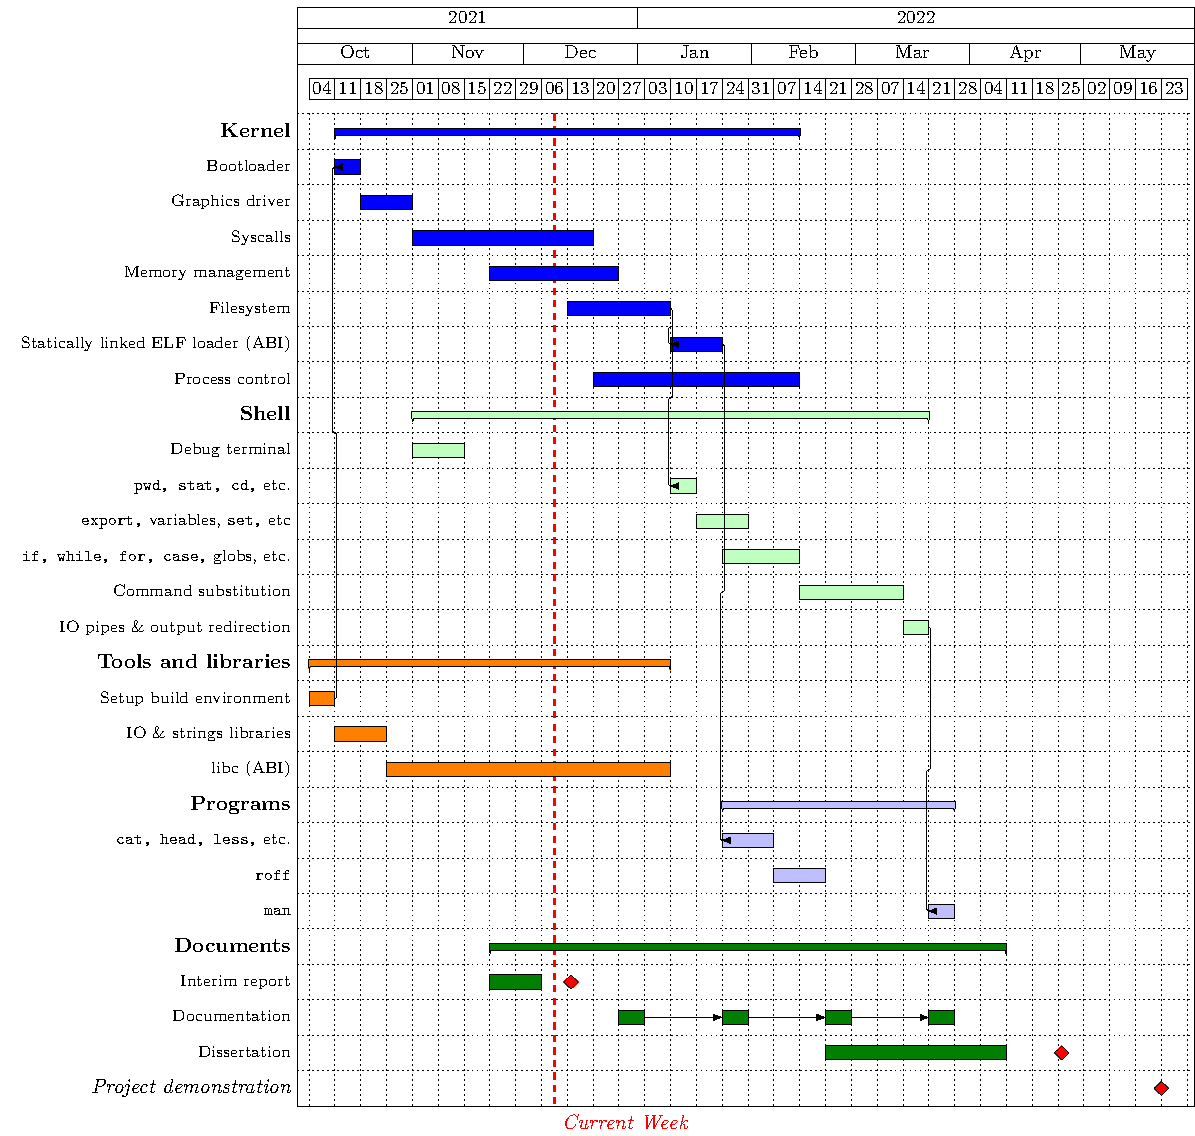
\includegraphics[width=0.8\textwidth]{build/interim-gantt.pdf}
    \caption{The Gantt chart}
    \label{fig:interim_gantt}
\end{figure}

\clearpage
\section{Project proposal tables and figures}
This appendix contains all of the tables, figures, and diagrams from the
original project proposal, laying out my initial beliefs about what the project
entailed, and how much work each part of the project would take.

The diagrams are copied directly from the project proposal, so tenses may now
be incorrect (e.g. ``I think'' instead of the now more correct ``I thought''),
but this is done intentionally as this section is included only as a reference
to the content of the previous document.

\subsection{Work tasks}
Tasks are the individual components of the project, separated into the
components of the Kernel and Shell, the miscellaneous parts, and the documents
I will need to produce for the project. These tasks are enumerated in
\autoref{tab:original-work-plan} and then assembled into a Gantt chart in
\autoref{fig:original-gantt-chart}.

\begin{table}[H]
\begin{center}
\begin{tabular}{|l|r|}
    \hline
    Task & Duration (weeks)\\
    \hline \textbf{Kernel} &\\
    Bootloader & 1\\
    Graphics driver & 2\\
    Syscalls & 6\\
    Filesystem & 3\\
    Statically linked ELF Loader & 2\\
    Memory management & 4\\
    Process control & 8\\
    Init system and service manager & 5\\
    Threads and multithreading & 4\\
    \hline \textbf{Shell} &\\
    Debug shell & 2\\
    \texttt{pwd}, \texttt{cd}, \texttt{ls}, \texttt{stat}, etc. & 2\\
    \texttt{export}, variables, \texttt{set}, etc. & 2\\
    \texttt{if}, \texttt{while}, \texttt{for}, \texttt{case}, globs, etc. & 3\\
    Command substitution & 4\\
    IO pipes and output redirection & 1\\
    \hline \textbf{Misc parts} &\\
    Setup cross-compiler and build environment & 1\\
    IO and strings libraries & 2\\
    libc & 8\\
    \texttt{cat}, \texttt{head}, \texttt{less}, etc. & 2\\
    \texttt{roff} & 1\\
    \texttt{man} & 1\\
    \hline \textbf{Documents} &\\
    Interim report & 1\\
    Documentation & 5\\
    Dissertation & 7\\
    \hline
\end{tabular}
\caption{The original plan of work for the project, including how many weeks I
thought each component would take.}
\label{tab:original-work-plan}
\end{center}
\end{table}

\subsection{Gantt chart}
\begin{figure}[H]
    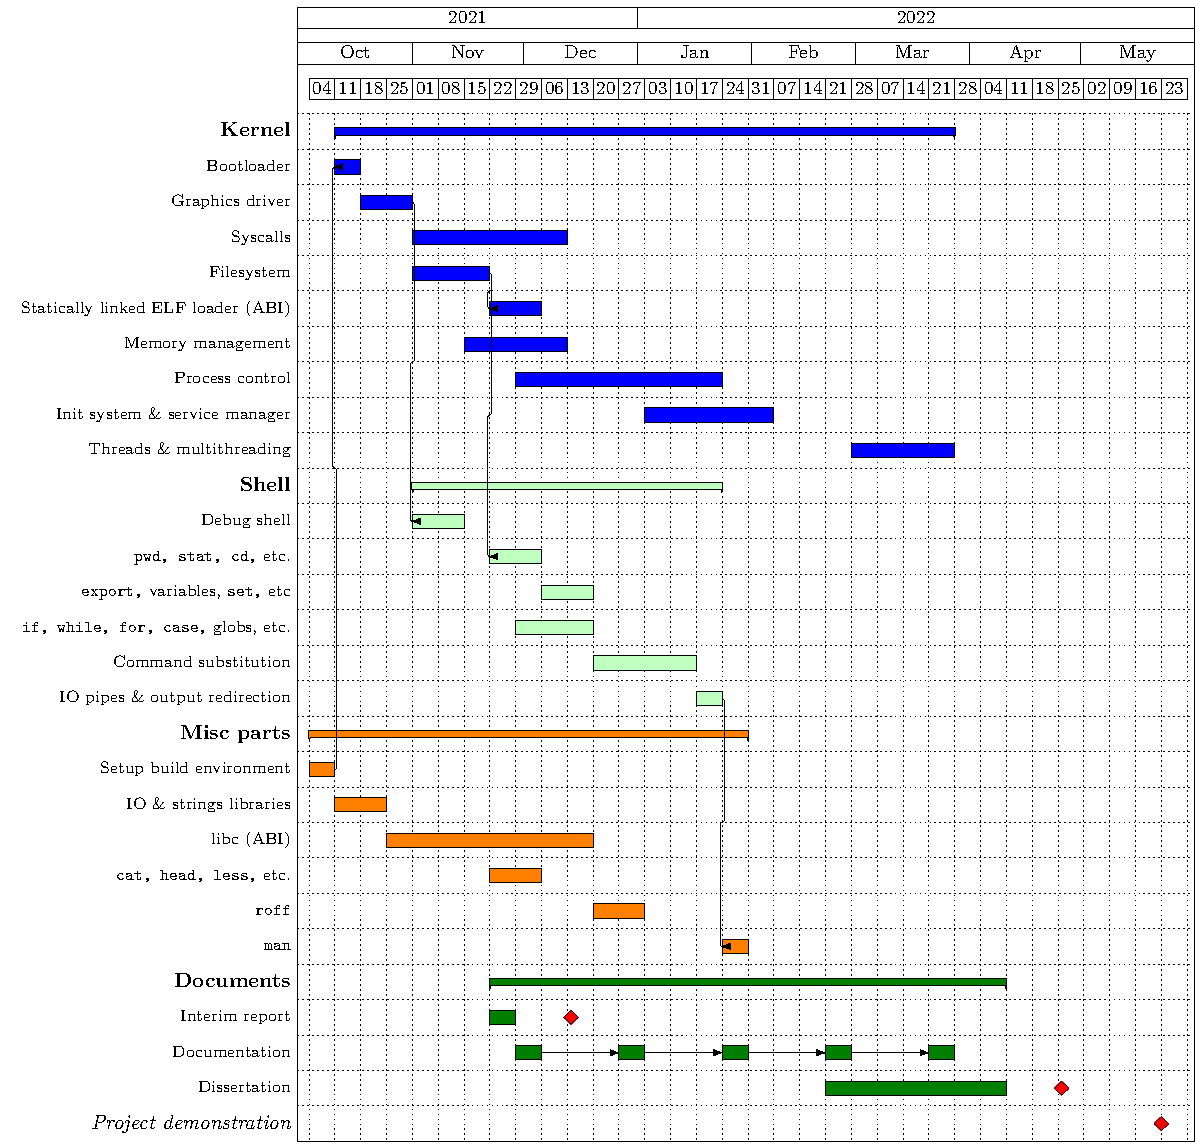
\includegraphics[width=0.95\textwidth]{build/original-gantt.pdf}
    \caption{A Gantt chart breaking down the proposed schedule of work for this
    project.}
    \label{fig:original-gantt-chart}
\end{figure}

\subsection{Work Packages}
A ``Work Package'' is a collection of tasks with a well-defined deliverable.
Not every task will be part of a work package, and some tasks will be work
packages on their own. \autoref{tab:original-work-packages} contains all of the
work packages for this project.

\begin{table}[H]
\begin{center}
\begin{tabular}{|p{40mm}|p{115mm}|}
    \hline
    \textbf{Work package} & \textbf{Description of the deliverable} \\
    \hline
    Debug shell using the graphics driver &
    A debug shell which is printed on the \gls{rpi}'s display and which uses
    keyboard input. The debug shell should accept several commands for
    debugging the processor status (including, but not limited to, printing the
    contents of memory, writing to memory, and jumping to a given memory
    address).
    \\ \hline
    A basic kernel which can load (from disk) and jump into a compiled \gls{elf}
    program. &
    A program that can load a statically compiled \gls{elf} executable binary
    into memory and then jump to its entry point. This requires a filesystem
    library to be implemented, and also includes the \gls{elf} loader task.
    \\ \hline
    Scheduling algorithm &
    A scheduling algorithm with support for multiple processes running on the
    system concurrently. This will include an implementation of
    \texttt{fork(3)} or a similar function in order to spawn new processes and
    \texttt{execve(2)} to replace the current program with a new process.
    \\ \hline
    Init system and service manager &
    An init system which is run at boot and starts all necessary parts of the
    \gls{os} and then spawns the root shell. The service manager ensures that
    all desired daemons and processes are started at the correct times and
    remain running, restarting them if they die.
    \\ \hline
    A shell &
    A (POSIX-compliant) shell \textbf{or} a port of a simple shell like
    Dash\cite{dash-shell}. If I decide that implementing my own POSIX-compliant
    shell is too large of a task, then I will port the source code for Dash to
    run on my \gls{os}, implementing the required syscalls to get it working.
    This shell will be the main way users interact with the \gls{os}.
    \\ \hline
    Documentation &
    This package contains several parts. I will create documentation for how
    each part of the \gls{os} works, and a guide for how new programmers can get
    started developing programs for the system. The documentation will be
    completed in stages as I develop the \gls{os}, and I will go back
    to keep it up-to-date as I make changes to components and add new
    components.
    \\ \hline
    Multithreading support and multi-core scheduling &
    The \gls{rpi} 3 has 4 \gls{cpu} cores. This work package will enable users
    to take advantage of the additional processing power of the other 3 cores
    for their programs. This includes a threading library similar to
    \texttt{pthread} on Linux systems, and improvements to the scheduler so
    that it can give different \gls{cpu} cores to multiple threads owned by the
    same process. \textbf{This work package is optional}.
    \\ \hline
\end{tabular}
\caption{The work packages of the project and their deliverables.}
\label{tab:original-work-packages}
\end{center}
\end{table}

\section{Extra diagrams}

\begin{figure}[H]
    \centering
    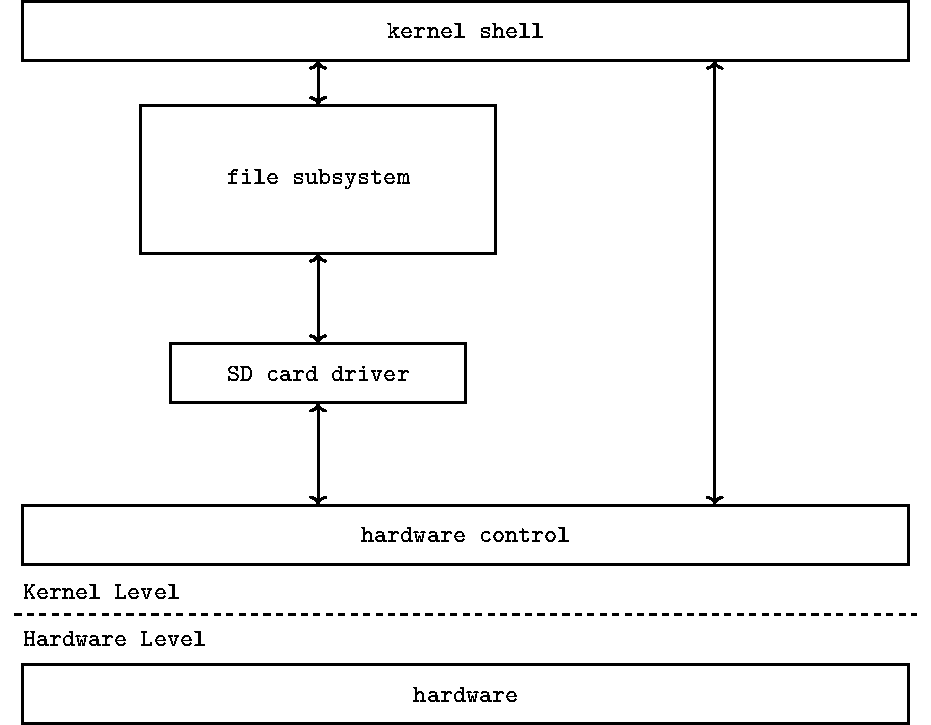
\includegraphics[width=0.8\textwidth]{build/finished-block-diagram.pdf}
    \caption{The current structure of the \gls{os}.}
    \label{fig:appendix_finished_block_diagram}
\end{figure}

\begin{figure}[H]
    \centering
    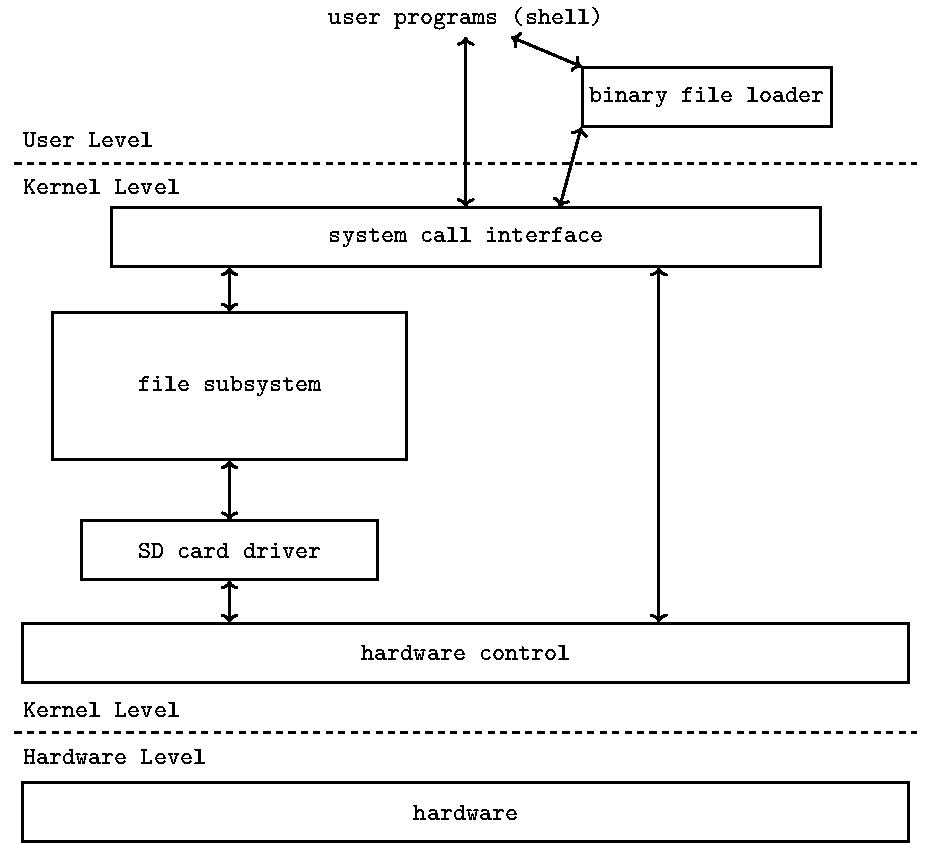
\includegraphics[width=0.8\textwidth]{build/nextstep-block-diagram.pdf}
    \caption{The `next-step' for the \gls{os} if it was aiming to become Unix
    after the end of this project.}
    \label{fig:appendix_nextstep_block_diagram}
\end{figure}

\begin{figure}[H]
    \centering
    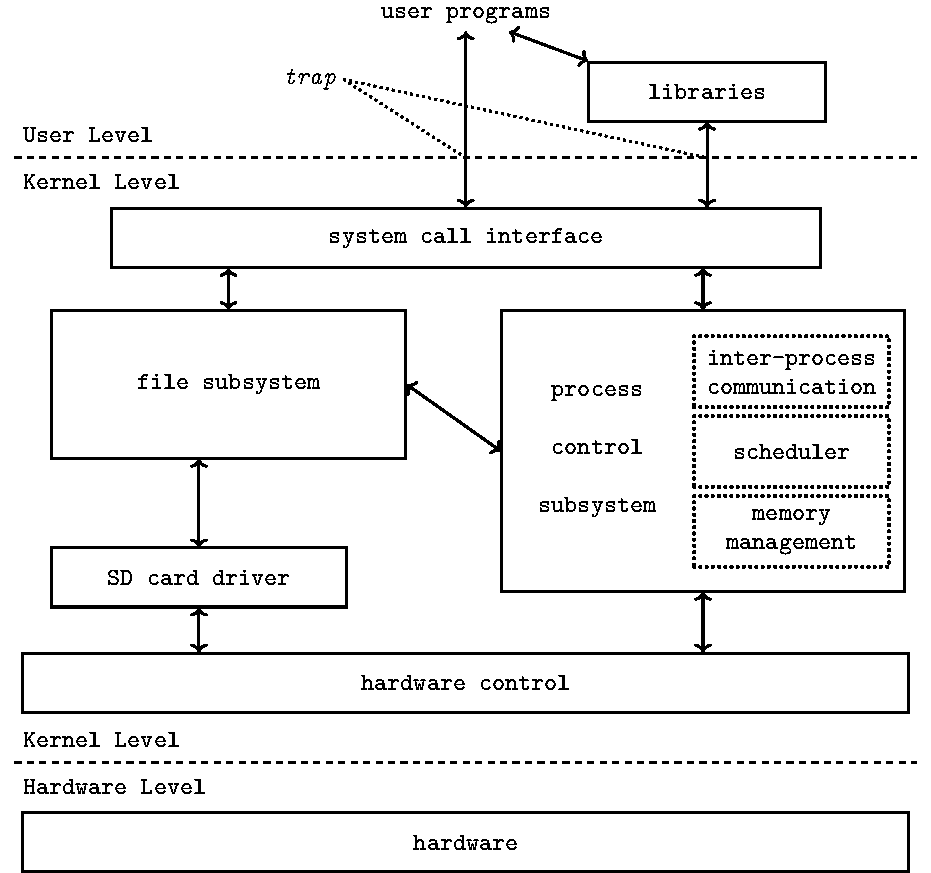
\includegraphics[width=0.8\textwidth]{build/os-block-diagram.pdf}
    \caption{The structure of the Unix \gls{os}.}
    \label{fig:appendix_os_block_diagram}
\end{figure}

\section{Shell future ideas}

Here are some `honorable mentions' which didn't make it into the main report.

\begin{itemize}
    \item Support for arrow-key navigation (and other special non-character
        keys) in the console input line
        \begin{itemize}
            \item History of previous lines entered into the console with
                up-arrow to get the previous line
            \item Cursor position on the line (cursor is between two
                characters)
            \item Backspace to delete one character back, delete to delete one
                character forwards
        \end{itemize}
    \item Text pager, like \texttt{less} or \texttt{more}
\end{itemize}


\clearpage
% End of main document - print glossaries, references, etc.
\printglossaries


\end{document}
